% Versão 24/06/2020

% Este documento destina-se a servir como modelo para a produção de documentos
% de pesquisa do PPGINF/UFPR, como projetos, dissertações e teses. A classe de
% documento se chama "ppginf" (arquivo ppginf.cls) e define o formato básico do
% documento. O texto está organizado em capítulos que são colocados em
% subdiretórios separados. São definidos exemplos para a inclusão de figuras,
% códigos-fonte e a definição de tabelas.
%
% Produzido por Carlos Maziero (maziero@inf.ufpr.br).

%=====================================================

% Opções da classe ppginf:
%
% - defesa    : versão para entregar à banca; tem espaçamento 1,5
%               e omite algumas páginas iniciais (agradecimentos, etc)
% - final     : versão pós-defesa, para enviar à biblioteca;
%               tem espaçamento simples e todas as páginas iniciais.
% - oneside   : somente frente; use quando for gerar somente o PDF.
% - twoside   : frente/verso; use se precisar de uma versão impressa.
% - metadados : inclui metadados no PDF (por default não inclui)
% - ...       : demais opções aceitas pela classe "book"

% ATENÇÂO: este modelo tem suporte para português e inglês.
% As duas línguas devem ser informadas como opção da classe;
% a língua principal do documento deve vir POR ÚLTIMO.

% Versão de defesa
%\documentclass[defesa,oneside,english,brazilian]{ppginf}

% Versão de defesa em inglês
%\documentclass[defesa,oneside,brazilian,english]{ppginf}

% Versão final em PDF para a biblioteca da UFPR
%\documentclass[final,oneside,english,brazilian]{ppginf}

% Versão final para impressão (frente/verso)
\documentclass[final,twoside,english,brazilian]{ppginf}

% configurações de diversos pacotes, inclusive a fonte usada no texto
% Pacotes usados neste documento e suas respectivas configurações

% ------------------------------------------------------------------------------

% Definição de fontes

% formato dos arquivos-fonte (utf8 no Linux e latin1 no Windows)
\usepackage[utf8]{inputenc}	% arquivos LaTeX em Unicode (UTF8)

% usar codificação T1 para ter caracteres acentuados corretos no PDF
\usepackage[T1]{fontenc}

% fonte usada no corpo do texto (descomente apenas uma)
\usepackage{newtxtext,newtxmath}	% Times (se não tiver, use mathptmx)
%\usepackage{lmodern}			% Computer Modern (fonte clássico LaTeX)
%\usepackage{kpfonts}			% Kepler/Palatino (idem, use mathpazo)
%\renewcommand{\familydefault}{\sfdefault} % Arial/Helvética (leia abaixo)

% A biblioteca central da UFPR recomenda usar Arial, seguindo a recomendação da
% ABNT. Essa é uma escolha ruim, pois fontes sans-serif são geralmente inade-
% quados para textos longos e impressos, sendo melhores para páginas Web.
% http://www.webdesignerdepot.com/2013/03/serif-vs-sans-the-final-battle/.

% fontes usadas em ambientes específicos
\usepackage[scaled=0.9]{helvet}		% Sans Serif
\usepackage{courier}			% Verbatim, Listings, etc

% ------------------------------------------------------------------------------

% inclusão de figuras em PDF, PNG, PS, EPS
\usepackage{graphicx}

% subfiguras (subfigure is deprecated, don't use it)
\usepackage[labelformat=simple]{subcaption}
\renewcommand\thesubfigure{(\alph{subfigure})}

% ------------------------------------------------------------------------------

% inclusão/formatação de código-fonte (programas)
\usepackage{listings}
\lstset{language=c}
\lstset{basicstyle=\ttfamily\footnotesize,commentstyle=\textit,stringstyle=\ttfamily}
\lstset{showspaces=false,showtabs=false,showstringspaces=false}
\lstset{numbers=left,stepnumber=1,numberstyle=\tiny}
\lstset{columns=flexible,mathescape=true}
\lstset{frame=single}
\lstset{inputencoding=utf8,extendedchars=true}
\lstset{literate={á}{{\'a}}1  {ã}{{\~a}}1 {à}{{\`a}}1 {â}{{\^a}}1
                 {Á}{{\'A}}1  {Ã}{{\~A}}1 {À}{{\`A}}1 {Â}{{\^A}}1
                 {é}{{\'e}}1  {ê}{{\^e}}1 {É}{{\'E}}1  {Ê}{{\^E}}1
                 {í}{{\'\i}}1 {Í}{{\'I}}1
                 {ó}{{\'o}}1  {õ}{{\~o}}1 {ô}{{\^o}}1
                 {Ó}{{\'O}}1  {Õ}{{\~O}}1 {Ô}{{\^O}}1
                 {ú}{{\'u}}1  {Ú}{{\'U}}1
                 {ç}{{\c{c}}}1 {Ç}{{\c{C}}}1 }

% ------------------------------------------------------------------------------

% formatação de algoritmos
\usepackage{algorithm,algorithmic}
\iflanguage{brazilian} {\floatname{algorithm}{Algoritmo}}{}
\renewcommand{\algorithmiccomment}[1]{~~~// #1}
%\algsetup{linenosize=\footnotesize,linenodelimiter=.}

% ------------------------------------------------------------------------------

% listas de símbolos e de abreviações (a fazer)
%\usepackage[titles]{tocloft}
%\newlistof[part]{symb}{los}{Lista de Símbolos}
%\newlistof[part]{abbrev}{loa}{Lista de Abreviações}
%\newcommand{\symb}[2]{%
%\refstepcounter{symb}
%\addcontentsline{los}{symb}{\protect #1 :#2}\par}

% ------------------------------------------------------------------------------

% formatação de bibliografia
\usepackage{natbib}		% bibliografia no estilo NatBib

% ------------------------------------------------------------------------------

% outros pacotes diversos
\usepackage{alltt,moreverb}	% mais comandos no modo verbatim
\usepackage{lipsum}		% gera texto aleatório (para os exemplos)
\usepackage{currfile}		% infos sobre o arquivo/diretório atual
\usepackage[final]{pdfpages}	% inclusão de páginas em PDF
\usepackage{longtable}		% tabelas multi-páginas (tab símbolos/acrônimos)

% ------------------------------------------------------------------------------



%=====================================================

\begin {document}

% Principais dados, usados para gerar as páginas iniciais.
% Campos não utilizados podem ser removidos ou comentados.

% título
\title{Sistemas de armazenamento de energia para microrredes e veículos elétricos}

% palavras-chave e keywords (p/ resumo, abstract e metadados do PDF)
%\pchave{Palavra-chave 1. Palavra-chave 2. Palavra-chave 3.}
%\keyword{Keyword 1. Keyword 2. Keyword 3.}

% autoria
\author{Gabriel Janetzky Pensky}
\advisor{Rogers Demonti}
%\coadvisor{Leslie Lamport}

% instituição
\IfLanguageName{brazilian}
  { \instit{UFPR}{Universidade Federal do Paraná} }
% a Bib/UFPR exige que tudo seja em português, exceto o título :-(
%  { \instit{UFPR}{Federal University of Paraná} }
  { \instit{UFPR}{Universidade Federal do Paraná} }

% área de concentração (default do PPGInf, não mudar)
%\IfLanguageName{brazilian}
%  { \field{Ciência da Computação} }
% a Bib/UFPR exige que tudo seja em português, exceto o título :-(
%  { \field{Computer Science} }
%  { \field{Ciência da Computação} }

% data (só o ano)
\date{2020}

% local
\IfLanguageName{brazilian}
  { \local{Curitiba PR} }
% a Bib/UFPR exige que tudo seja em português, exceto o título :-(
%  { \local{Curitiba PR - Brazil} }
  { \local{Curitiba PR} }

% imagem de fundo da capa (se não desejar, basta comentar)
\coverimage{0-iniciais/fundo-capa.jpg}

%=====================================================

%% Descrição do documento (obviamente, descomentar somente UMA!)

% Por exigência da biblioteca da UFPR, a descrição do documento deve ser
% em português, mesmo em documentos em outras línguas. Vá entender...

% tese de doutorado
%\descr{Tese apresentada como requisito parcial à obtenção do grau de Doutor em Ciência da Computação no Programa de Pós-Graduação em Informática, Setor de Ciências Exatas, da Universidade Federal do Paraná}

% exame de qualificação de doutorado
%\descr{Documento apresentado como requisito parcial ao exame de qualificação de Doutorado no Programa de Pós-Graduação em Informática, Setor de Ciências Exatas, da Universidade Federal do Paraná}

% dissertação de mestrado
%\descr{Dissertação apresentada como requisito parcial à obtenção do grau de Mestre em Informática no Programa de Pós-Graduação em Informática, Setor de Ciências Exatas, da Universidade Federal do Paraná}

% exame de qualificação de mestrado
%\descr{Documento apresentado como requisito parcial ao exame de qualificação de Mestrado no Programa de Pós-Graduação em Informática, Setor de Ciências Exatas, da Universidade Federal do Paraná}

% trabalho de conclusão de curso
%\descr{Trabalho apresentado como requisito parcial à conclusão do Curso de Bacharelado em XYZ, Setor de Ciências Exatas, da Universidade Federal do Paraná}

% relatório final de IC
\descr{Relatório apresentado à Coordenação de Iniciação Científica e Tecnológica da Universidade Federal do Paraná como requisito parcial da conclusão das atividades de Iniciação Científica ou Iniciação em desenvolvimento tecnológico e Inovação - Edital 2019}

% trabalho de disciplina
%\descr{Trabalho apresentado como requisito parcial à conclusão da disciplina XYZ no Curso de Bacharelado em XYZ, Setor de Ciências Exatas, da Universidade Federal do Paraná}

% doctorate thesis
%\descr{Thesis presented as a partial requirement for the degree of Doctor in Computer Science in the Graduate Program in Informatics, Exact Sciences Sector, of the Federal University of Paraná, Brazil}

% doctorate qualification
%\descr{Document presented as a partial requirement for the doctoral qualification exam in the Graduate Program in Informatics, Exact Sciences Sector, of the Federal University of Paraná, Brazil}

% MSc dissertation
%\descr{Dissertation presented as a partial requirement for the degree of Master of Sciences in Informatics in the Graduate Program in Informatics, Exact Sciences Sector, of the Federal University of Paraná, Brazil.}

% MSc qualification
%\descr{Document presented as a partial requirement for the Master of Sciences qualification exam in the Graduate Program in Informatics, Exact Sciences Sector, of the Federal University of Paraná, Brazil}

%=====================================================

% define estilo das páginas iniciais (capas, resumo, sumário, etc)
\frontmatter
\pagestyle{frontmatter}

% produz capa e folha de rosto
\titlepage

% páginas que só aparecem na versão final (a inclusão é automática)
%% IMPORTANTE: o conteúdo exato da ficha catalográfica é preparada pela
% Biblioteca da UFPR. Não "invente" um conteúdo para ela!

\begin{ficha}	% só gera conteúdo se for na versão final

% inclusão da ficha catalográfica final (arquivo PDF)
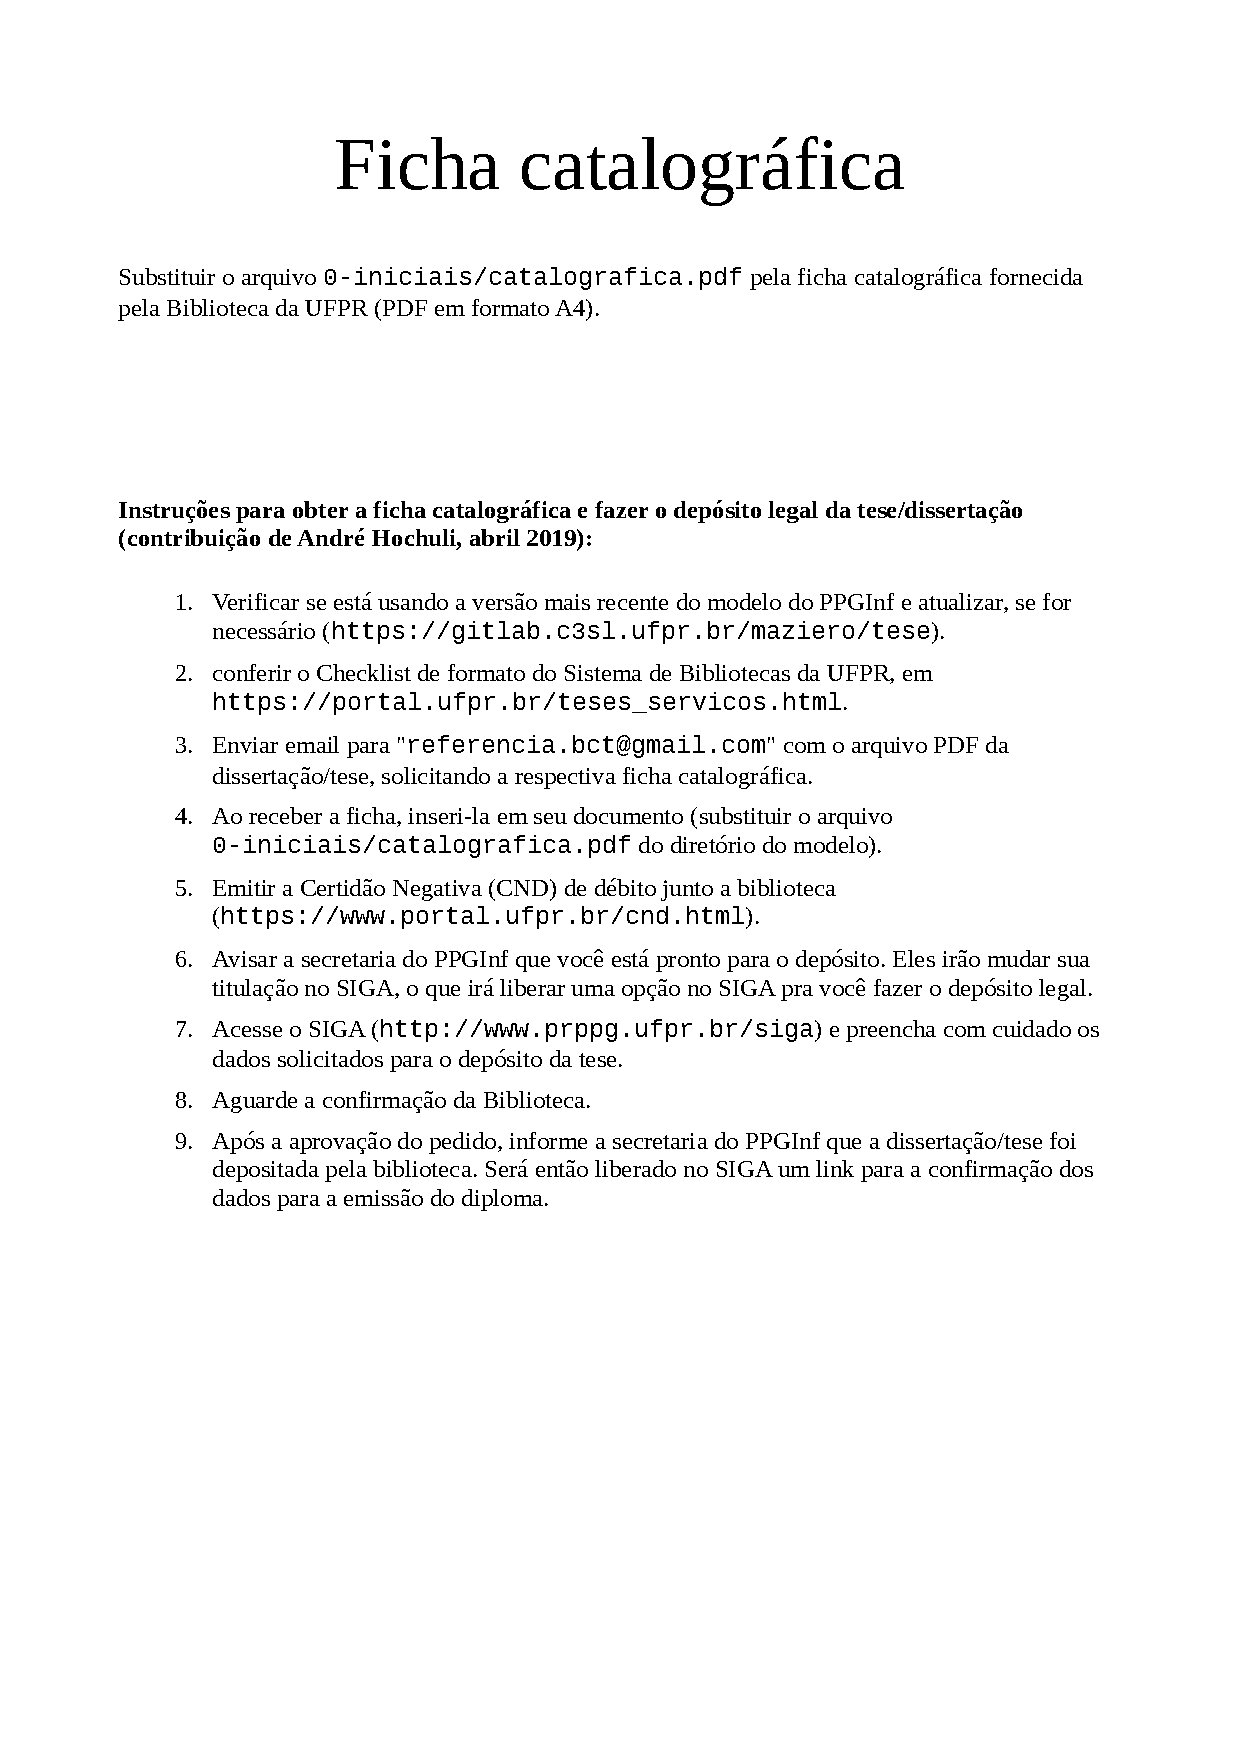
\includepdf[noautoscale]{0-iniciais/catalografica.pdf}

\end{ficha}

%=====================================================
	% ficha catalográfica
%% A ficha de aprovação será fornecida pela secretaria do programa,
% após a defesa e cumprimento dos demais trâmites legais.

\begin{aprovacao}	% só gera conteúdo se for na versão final

% inclusão do termo de aprovação final (arquivo PDF)
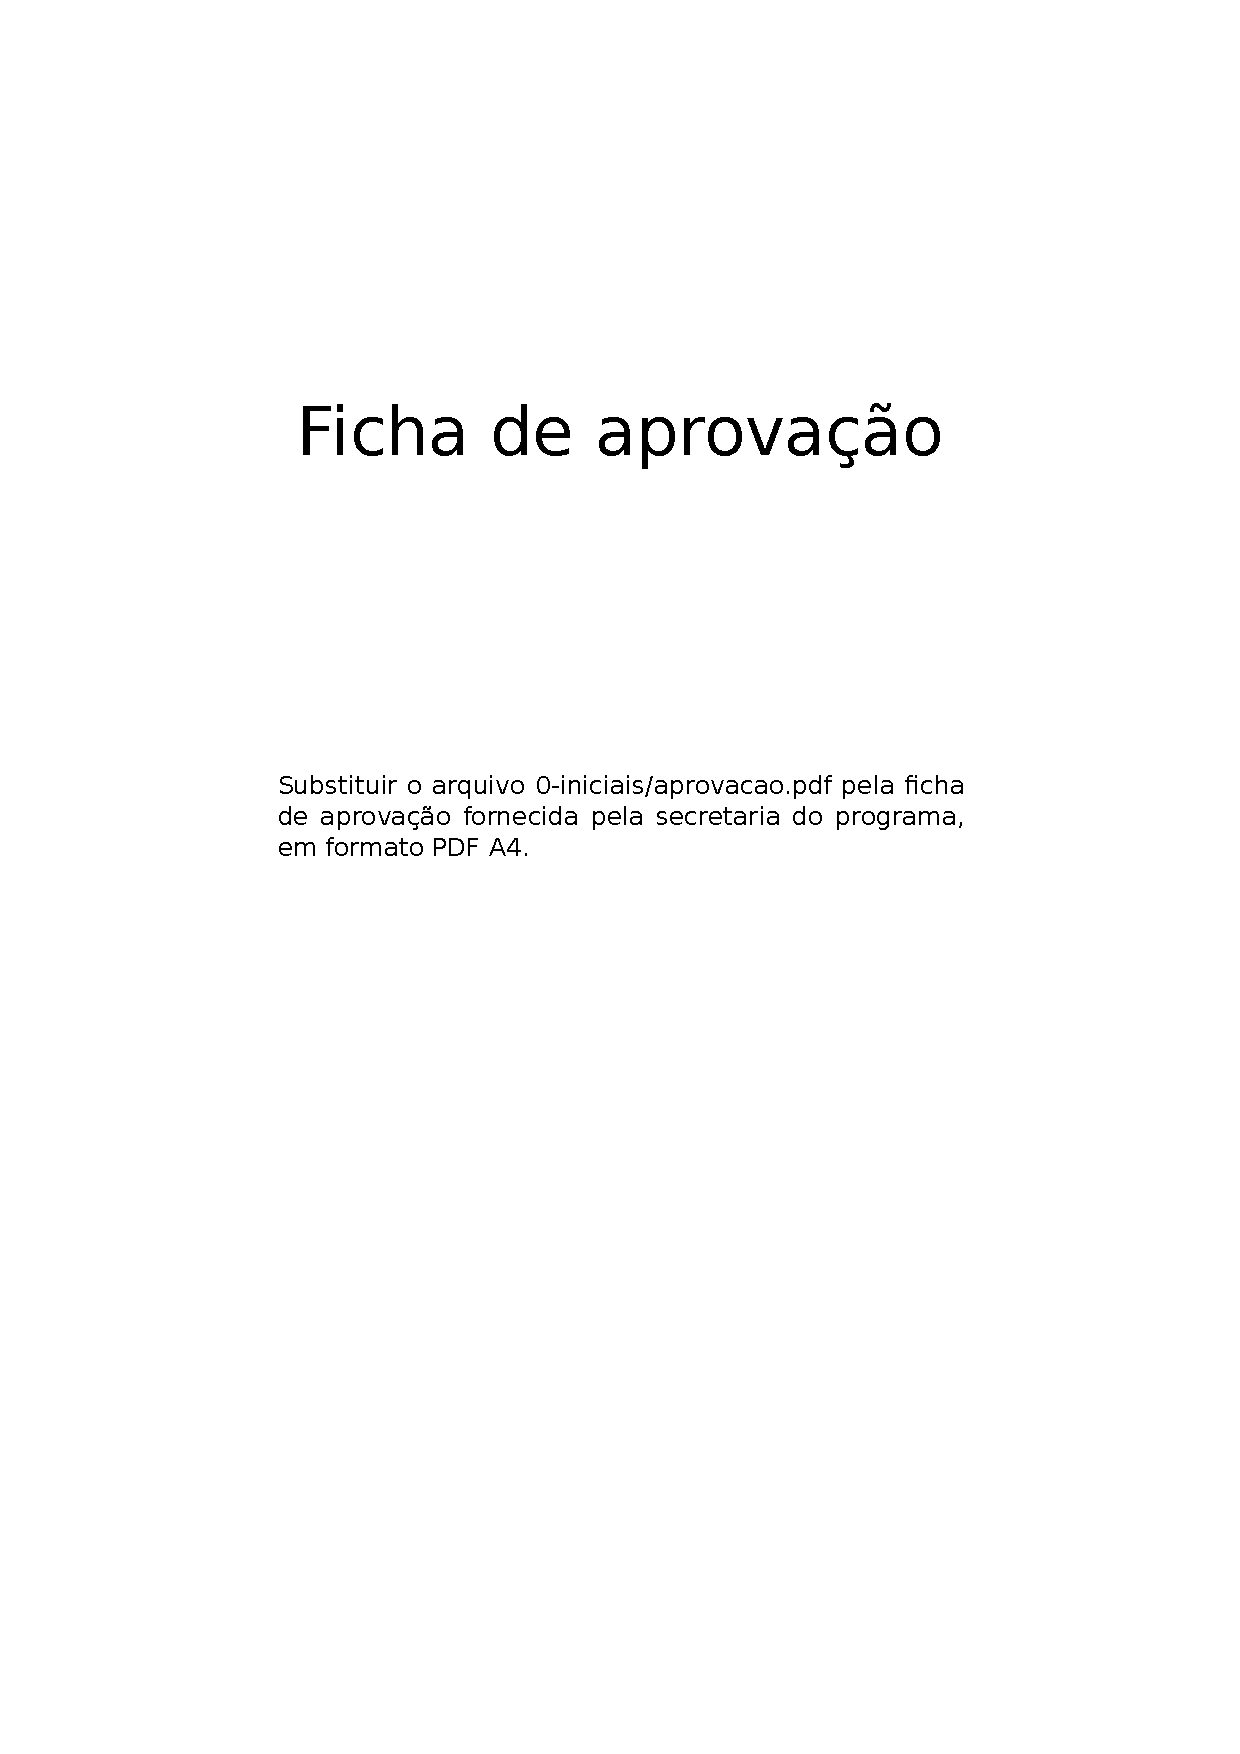
\includepdf[noautoscale]{0-iniciais/aprovacao.pdf}

\end{aprovacao}

%=====================================================
		% folha de aprovação
%\begin{dedica}  % só gera conteúdo se for na versão final

A alguém...

\end{dedica}

		% dedicatória
%\begin{agradece}	% só gera conteúdo se for na versão final

Inserir os agradecimentos. Os agradecimentos devem ocupar no máximo uma página, devem ser justificados na largura da página e com um afastamento de parágrafo na primeira linha de 1,27 cm. O espaçamento entre linhas deve ser de 1,5 linhas. Não deve haver espaçamento adicional entre parágrafos.

\lipsum[2-5]	% gera um texto aleatório

\end{agradece}

		% agradecimentos

% resumo (português) e abstract (inglês)
\begin{resumo}

Uma crescente preocupação com fatores climáticos e com o aquecimento global visando uma diminuição do consumo de combustíveis fósseis, vem abrindo espaço para o desenvolvimento de novos modelos na geração e consumo de energia. Uma evolução das fontes renováveis de energia trouxe a possibilidade de uma geração descentralizada, surgindo assim, o conceito da microrrede. Essas, trazem novas necessidades na manutenção da qualidade e no controle da energia elétrica em redes com geração intermitente, levando assim, ao uso de sistemas de armazenamento de energia. Além disso, o avanço na mobilidade elétrica, proporcionando uma maior densidade de energia das baterias, possibilitou o surgimento de veículos elétricos baratos e competitivos.

Desta forma, o objetivo deste trabalho foi o desenvolvimento de dois sistemas de armazenamento de energia, um conectado à microrrede do Departamento de Engenharia Elétrica (DELT) localizado no Centro Politécnico da Universidade Federal do Paraná (UFPR) em Curitiba e outra utilizada em um veículo elétrico do tipo Formula SAE, para competição nacional pela equipe UFPR Formula.

Primeiramente foi feito um estudo dos sistemas nos quais o armazenamento seria integrado, com uma revisão teórica do funcionamento dos principais componentes; foi então feito um estudo dos diferentes tipos e tecnologias de sistemas de armazenamento de energia, suas aplicações, características, estado da arte e aspectos de segurança; uma metodologia de organização do projeto foi definida: inicialmente definidos requerimentos para cada subsistema, depois projeto da arquitetura e integração do sistema, chegando na especificação do componente; e finalmente, como resultado se teve um projeto completo e especificado para os dois sistemas.

\end{resumo}

%\begin{otherlanguage}{english}

\begin{abstract}

% em inglês, o primeiro parágrafo não deve ser indentado
\noindent
The abstract should be the English translation of the ``resumo'', no more, no less.

\end{abstract}

\end{otherlanguage}



% listas  de figuras, tabelas, abreviações/siglas, símbolos
\listoffigures				% figuras
\clearpage
\listoftables				% tabelas
%%=====================================================

% lista de acrônimos (siglas e abreviações)

\begin{listaacron}

\begin{longtable}{p{0.2\linewidth}p{0.7\linewidth}}
DINF & Departamento de Informática\\
PPGINF & Programa de Pós-Graduação em Informática\\
UFPR & Universidade Federal do Paraná\\
\end{longtable}

\end{listaacron}

%=====================================================
		% acrônimos, deve ser preenchida à mão
%%=====================================================

% lista de símbolos

\begin{listasimb}

\begin{longtable}{p{0.2\linewidth}p{0.7\linewidth}}
$\alpha$ & alfa, primeira letra do alfabeto grego\\
$\beta$ & beta, segunda letra do alfabeto grego\\
$\gamma$ & gama, terceira letra do alfabeto grego\\
$\omega$ & ômega, última letra do alfabeto grego\\
$\pi$ & pi \\
$\tau$ & Tempo de resposta do sistema\\
$\theta$ & Ângulo de incidência do raio luminoso\\
\end{longtable}

\end{listasimb}

%=====================================================
		% símbolos, idem
\tableofcontents			% sumário

%=====================================================

% define estilo do corpo do documento (capítulos e apêndices)
\mainmatter
\pagestyle{mainmatter}

% inclusao de cada capítulo, alterar a gosto (do professor de Metodologia)
\chapter{Introdução}

%=====================================================

% A introdução geral do documento pode ser apresentada através das seguintes seções: Desafio, Motivação, Proposta, Contribuição e Organização do documento (especificando o que será tratado em cada um dos capítulos). O Capítulo 1 não contém subseções\footnote{Ver o Capítulo \ref{cap-exemplos} para comentários e exemplos de subseções.}.

Este modelo foi proposto com o intuito de padronizar e simplificar as monografias, dissertações e teses produzidas no Departamento de Informática da UFPR. Ele foi vagamente inspirado nas normas da ABNT (conforme indicado em \cite{bibufpr15}), mas não as segue \emph{ipsis litteris}. Várias alterações foram feitas com o objetivo de melhorar sua estética e tornar o texto mais legível para trabalhos na área de informática. A versão atualizada deste modelo está disponível em \cite{maziero15}.

Este modelo está baseado em uma classe especifica \verb#ppginf.cls#, que aceita várias opções de compilação. A versão do documento pode ser:

\begin{itemize}

\item \verb#defesa#: é gerado um documento em espaço 1,5, frente simples e sem as páginas iniciais adicionais; é uma versão adequada para receber as anotações dos membros da banca de defesa.

\item \verb#final#: é gerado um documento em espaço simples, frente/verso, com páginas iniciais (capa, ficha catalográfica, folha de aprovação, agradecimentos, etc). É uma versão bem mais compacta, mais ecológica e ideal para a impressão definitiva.

\end{itemize}

Para obter os melhores resultados, compile este modelo usando a seguinte sequência de passos:

\begin{quote}
\begin{footnotesize}
\begin{verbatim}
pdflatex  main          // compilação inicial
bibtex main             // processa referências bibliográficas
pdflatex  main          // compilação final
\end{verbatim}
\end{footnotesize}
\end{quote}

ou

\begin{quote}
\begin{footnotesize}
\begin{verbatim}
make                    // faz tudo...
\end{verbatim}
\end{footnotesize}
\end{quote}

Os principais itens considerados na formatação deste documento foram:

\begin{itemize}

\item Papel em formato A4, com margens de 20 mm à direita e embaixo, 30 mm nos demais lados. Não devem ser usados cabeçalhos ou rodapés além dos que estão aqui propostos.

\item O texto principal do documento escrito em 12 pontos. O fonte principal do texto pode ser selecionado no arquivo \verb#packages.tex#.

\item Código-fonte, listagens e textos similares são formatados em fonte Courier 12 ou 10 pontos.

\item O espaçamento padrão entre linhas é 1,5 linhas (1 linha na versão final). Não inserir espaços adicionais entre parágrafos normais. Figuras, tabelas, listagens e listas de itens devem ter um espaço adicional antes e após os mesmos.

\item As páginas iniciais não são numeradas.

\item O corpo do texto é numerado com algarismos arábicos (1, 2, 3, ...) a partir da introdução, ate o final do documento. Os números de página devem estar situados no alto à direita (páginas direitas) ou à esquerda (páginas esquerdas).

\item Expressões em inglês, grego, latim ou outras línguas devem ser enfatizadas em itálico, como \emph{sui generis} ou \emph{scheduling} (use o comando \verb#\emph{...}#).

\item Para reforçar algo, deve-se usar somente \textbf{negrito}. \underline{Sublinhado} ou MAIÚSCULAS não devem ser usados como forma de ênfase!

\item As notas de rodapé também têm um modelo\footnote{As notas de rodapé dever ser escritas em tamanho 10 pt, numeradas em arábico.}. Notas de rodapé servem para fazer algum comentário paralelo; não as use para colocar URLs, referências bibliográficas ou significado de siglas.

\end{itemize}

Felizmente o \LaTeX\ resolve a maior parte dessas questões!

%=====================================================
			% introdução
\chapter{Revisão da literatura}
\label{cap:exemplos}

% figuras estão no subdiretório "figuras/" dentro deste capítulo
\graphicspath{{\currfiledir/figuras/}}

%=====================================================

\section{A microrrede no Departamento de Engenharia Elétrica}

   O projeto da microrrede como um todo foi planejado para ser flexível com relação aos modos de operação, sendo possível utilizar conectado à rede de distribuição, quanto de forma isolada. Isso faz com que o fluxo de energia seja permitido nos dois sentidos. 

   \begin{figure}[!htb]
      \centering
      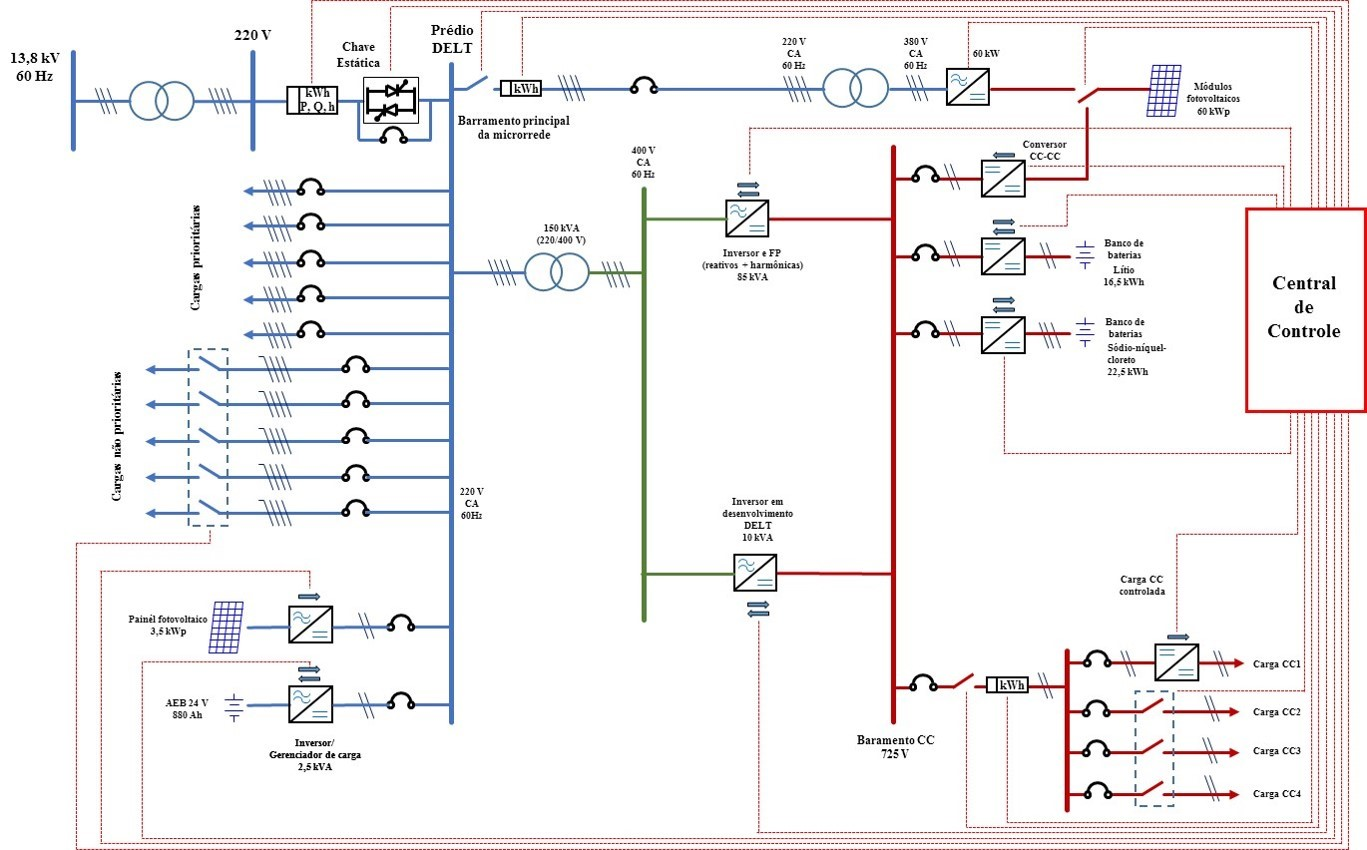
\includegraphics[width=\linewidth]{diagrama-microrrede.jpg}
      \caption{Diagrama completo da microrrede \cite{Dem19}.}
      \label{fig:diagrama-microrrede}
   \end{figure}

   A microrrede está localizada no laboratório de Eficiência Energética do Departamento de Engenharia Elétrica (DELT), no Centro Politécnico da UFPR. No diagrama da figura \ref{fig:diagrama-microrrede} podemos identificar os principais itens. Na subestação principal do compus se conecta um transformador de 350 kVA, na qual se ligam o prédio do departamento e outros prédios próximos com a tensão de 220 V. Após isso está o quadro de distribuição de energia geral. Continuando, temos uma chave eletrônica, responsável por fazer a desconexão da microrrede. 

   Parte da microrrede já está montada e é formada por um sistema de geração solar fotovoltaica de 3,5 kWp e um sistema de armazenamento de baterias de chumbo-ácido de capacidade total de 880 Ah em 24 V. Neste banco de armazenamento há um inversor e gerenciador de carga de 2,5 kW com capacidade de gerar um barramento estável monofásico em 127 V. Outros dispositivos instalados são as cargas formadas por diversos motores de indução acionando bombas d'agua, uma bomba de calor de 3 kW e um banco trifásico de capacitores com 10 kVAr.

   Está previsto ainda a instalação de três inversores, estes farão a conversão a energia proveniente de 208 módulos fotovoltaicos com um total de 65,5 kWp. Dois sistemas de armazenamento de energia serão utilizados no barramento CC de 725 V. Um será com baterias de sais de sódio-níquel-cloreto com capacidade de 22,5 kWh e os outro será com baterias de íons de lítio desenvolvidos nesse trabalho.

   Por último, ainda no barramento CC, serão conectadas várias cargas de corrente contínua, um conversor CC-CC de 30 kW e um conversor CC-CA de 85 kW. Este último é responsável pela conexão do barramento CC de 725 V em um barramento CA de 400 V. Um transformador de 150 kVA 220/400 V fará o acoplamento dos barramentos CA.

%=====================================================

\section{O carro elétrico da UFPR Formula 2020}

   Neste ano de 2020 o projeto do carro elétrico da equipe UFPR Formula está em sua terceira revisão. Nos últimos 2 anos foram usados dois motores a indução da fabricante brasileira WEG, assim como 2 inversores também da mesma fabricante. Estes tinham uma potência máxima de 20kW e nominal de 6kW cada. O sistema de armazenamento de energia utilizado em 2018 tinha 4,3 kWh, já em 2019 esse foi reduzido por vários aspectos de projeto, chegando a 3,4 kWh. Este conjunto garantia uma autonomia de cerca de 7 km.

   No projeto atual, o objetivo é se alcançar uma melhora de desempenho a ponto de competir no topo da competição nacional. Todo o projeto mecânico foi repensado pensando numa diminuição do peso e melhora da dinâmica do veículo. Já na parte elétrica, o sistema de tração foi inteiro renovado. O motor utilizado é um motor síncrono de fluxo axial da fabricante Emrax, com peso e tamanho reduzido, além de uma potência máxima de mais de 100 kW e nominal de 60 kW (a potência máxima na competição é limitada em 80 kW). O inversor é formado por um módulo de potência e um módulo de controle desenvolvido também no DELT por membros da equipe UFPR Formula. 

   Para se adequar ao novo projeto, a bateria foi inteira repensada e reprojetada. Uma nova tecnologia com maior densidade de potência e energia em relação à anterior foi escolhida, o nível de tensão foi aumentado para reduzir tamanho de componentes condutores e a capacidade foi drasticamente aumentada, para que fosse possível uma autonomia de pouco mais que 20 km (prova mais longa da competição).

%=====================================================

\section{Dispositivos fotovoltaicos}

   No uso de células fotovoltaicas, determinar o ponto de operação de máxima potência (\textit{Maximum Power Point – MPP}) é essencial para que toda a energia disponível seja utilizada \cite{Dem03}. A curva característica $I \times V$ de uma célula hipotética é apresentada a seguir (figura \ref{fig:curva-carac-fotovoltaica}), considerando a temperatura constante e em duas situações de insolação diferentes. Para que a máxima potência do módulo seja utilizada, ela deve operar nos pontos marcados como mpp. Pode-se observar que a localização do ponto no gráfico muda de acordo com a insolação, fazendo com que o controle da operação das células não seja trivial. Este controle normalmente é feito pelo dispositivo conversor acoplado às células fotovoltaicas.

   \begin{figure}[!htb]
      \centering
      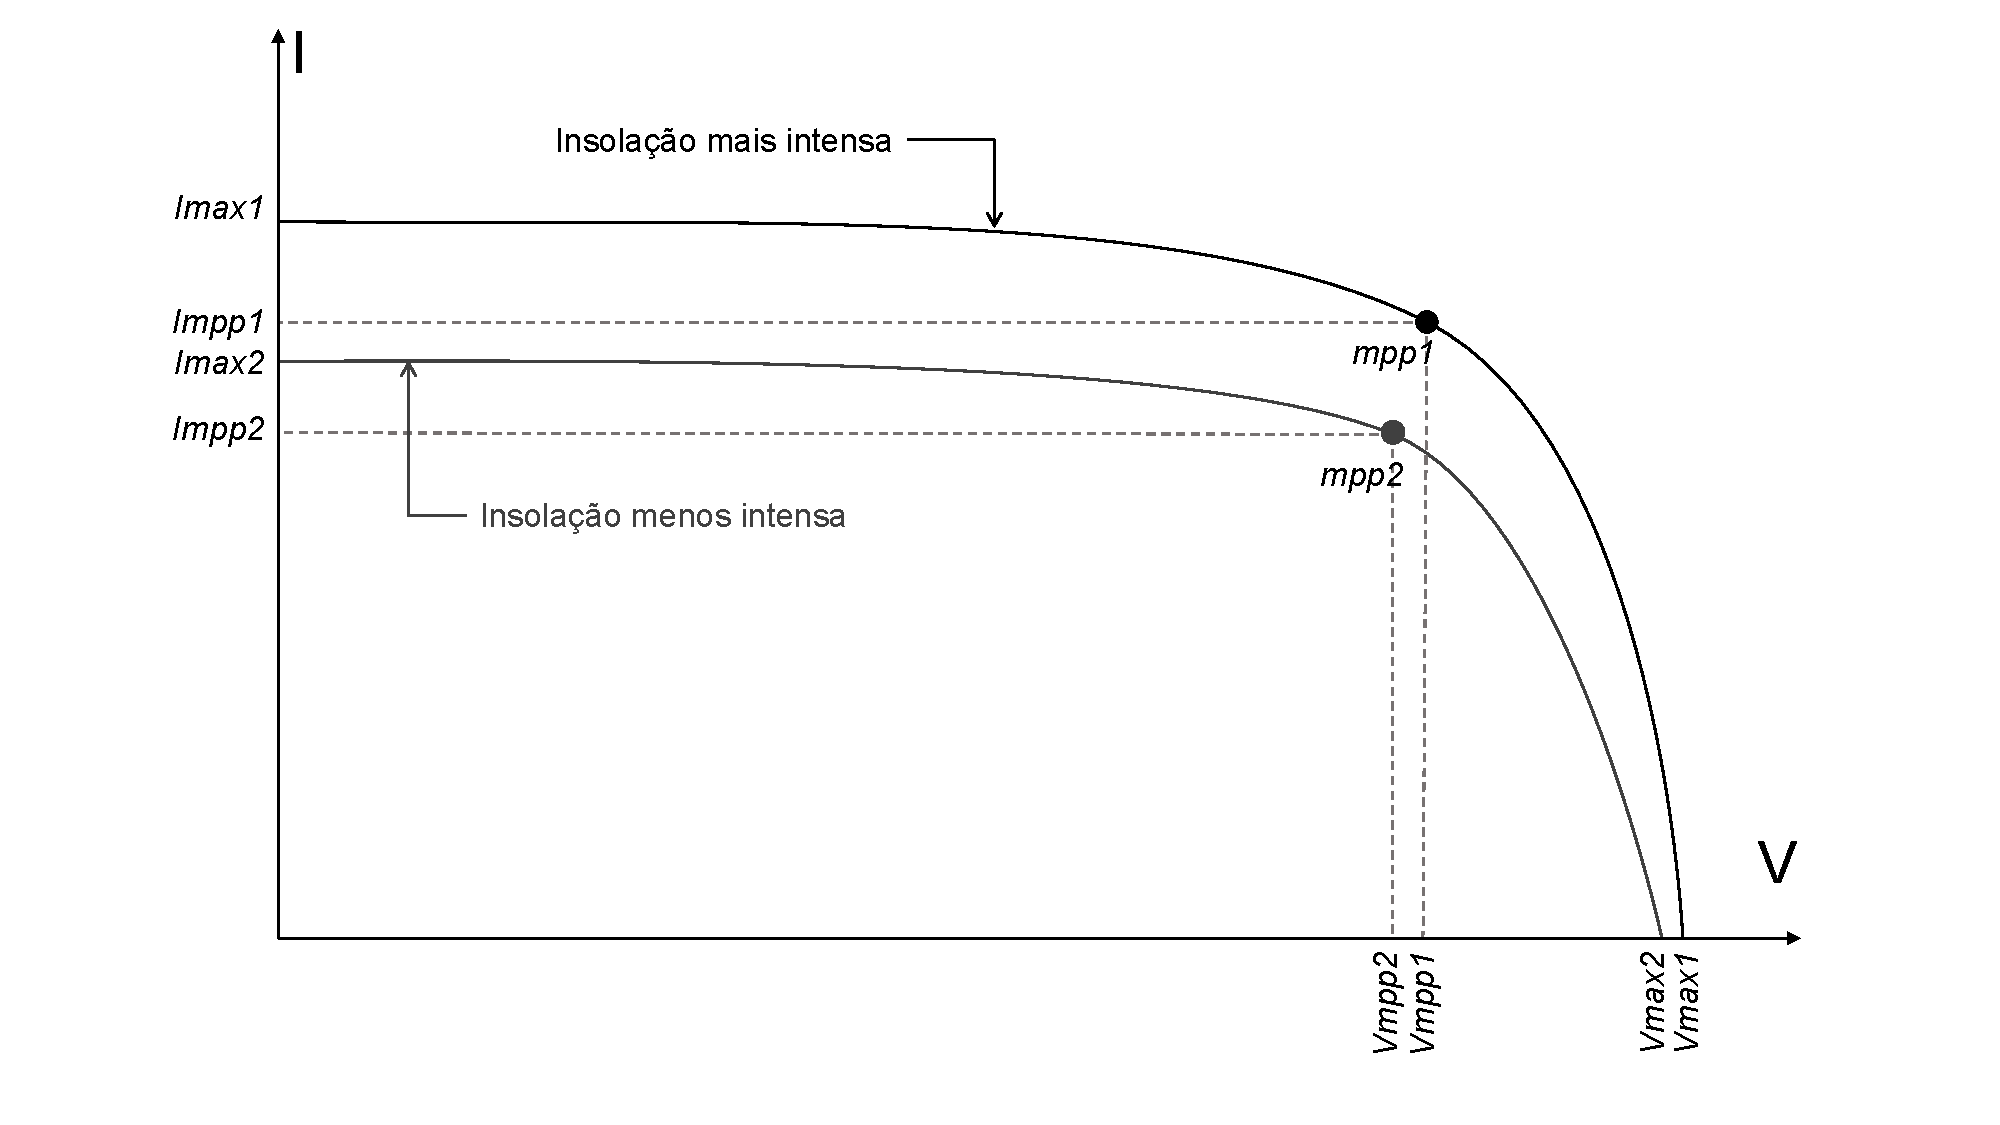
\includegraphics[width=14cm]{curva-carac-fotovoltaica.pdf}
      \caption{Curva $I \times V$ característica de célula fotovoltaica típica.}
   \label{fig:curva-carac-fotovoltaica}
   \end{figure}

   Além disso, podemos entender um dispositivo fotovoltaico pelo seu circuito equivalente, este é apresentado abaixo.

   \begin{figure}[!htb]
      \centering
      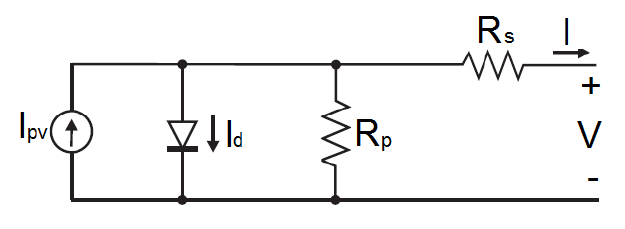
\includegraphics[height=3cm]{circ-eq-fotovoltaica.png}
      \caption{Circuito equivalente da célula fotovoltaica prática \cite{Oli16}.}
      \label{fig:circ-eq-fotovoltaica}
   \end{figure}

%=====================================================

\section{Conversores CC-CC}

   Conversores CC-CC são dispositivos formados por componentes passivos e semicondutores atuando como chave que têm por função controlar o fluxo de energia entre sua entrada e saída. Realizam isso convertendo a amplitude de tensão e corrente contínua da entrada em uma outra amplitude de saída, também em corrente contínua.

   Conversores simples têm por característica serem unidirecionais, podendo ser categorizados como abaixador, elevador ou abaixador-elevador de tensão. Considerado o conversor mais simples, o conversor abaixador de tensão, Buck, contém em sua forma mais reduzida um indutor ($L_o$), um diodo ($D$), um capacitor ($C_o$) e um semicondutor atuando como chave ($S$), como pode ser visto na figura \ref{fig:conv-buck}.

   O funcionamento exato não será discutido nesse trabalho, mas é importante saber que eles podem ser controlados pela ativação da chave $S$, alterando a frequência de ativação e outros parâmetros

   Além desses, outra categoria importante de conversor são os conversores bidirecionais, que têm por característica a habilidade de conduzir corrente nos dois sentidos, da entrada para a saída e da saída para a entrada. Uma das topologias mais simples é o conversor boost bidirecional apresentado na figura \ref{fig:conv-boost}.

   \begin{figure}[!htb]
   \centering
      \begin{subfigure}{0.48\linewidth}
         \centering
         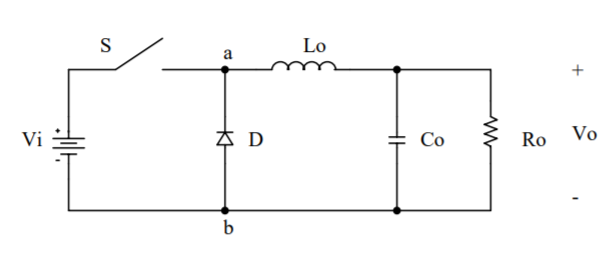
\includegraphics[height=4cm]{conv-buck.png}
         \caption{Conversor Buck \cite{Pet01}.}
         \label{fig:conv-buck}
      \end{subfigure}
      \hspace*{\fill}
      \begin{subfigure}{0.48\linewidth}
         \centering
         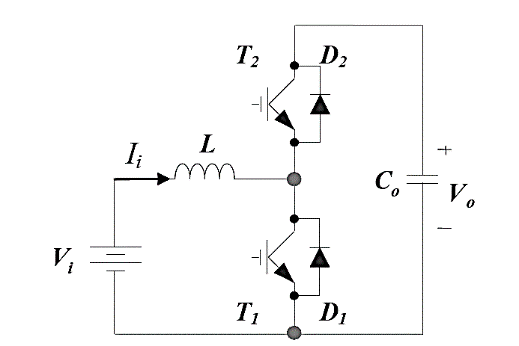
\includegraphics[height=4cm]{conv-boost.png}
         \caption{Conversor Boost \cite{Pom17}.}
         \label{fig:conv-boost}
      \end{subfigure}
   \caption{Conversores CC-CC citados.}
   \label{fig:conv-esquematicos}
   \end{figure}

%=====================================================

\section{Inversores}

   De forma semelhante aos conversores CC-CC, inversores são dispositivos formados por componentes passivos e semicondutores, mas que realizam a conversão da energia em corrente contínua para corrente alternada. É possível ainda que o sinal CA tenha uma ou mais fases, conforme necessidades do projeto. Para entendermos o funcionamento de um inversor podemos começar com o circuito mais simples: ponte H. Este é formado por apenas 4 chaves, que realizam a conexão entre a fonte e a carga (figura \ref{fig:inv-mono}). É um inversor monofásico, ou seja, gera apenas um sinal de corrente alternada de saída.

   Ele funciona invertendo a polaridade da carga conectada à fonte DC ao acionar de forma sincronizada duas chaves de cada vez, em um ciclo a chave $S1$ e $S4$, e em outro a chave $S2$ e $S3$, ou com todas as chaves abertas. Assim como os conversores CC-CC, o funcionamento não será investigado em detalhes. É importante sabermos que ele também funciona controlando a ativação das chaves com um sinal modulado na largura de pulso (PWM).

   Para que seja possível conectarmos inversores às redes de energia trifásicas ou máquinas trifásicas, precisamos também de um inversor trifásico. Este é muito semelhante à ponte H apresentada acima, mas conta com 6 chaves eletrônicas para gerar o sinal trifásico (figura \ref{fig:inv-tri}). As chaves também são acionadas de forma a gerar um sinal PWM de uma fonte senoidal, mas agora é possível que gere um sinal trifásico.

   \begin{figure}[!htb]
      \centering
         \begin{subfigure}{0.48\linewidth}
            \centering
            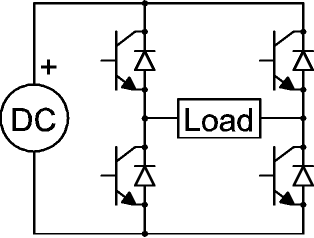
\includegraphics[height=4cm]{inv-mono.png}
            \caption{Inversor monofásico do tipo ponte H.}
            \label{fig:inv-mono}
         \end{subfigure}
         %\hspace*{\fill}
         \begin{subfigure}{0.48\linewidth}
            \centering
            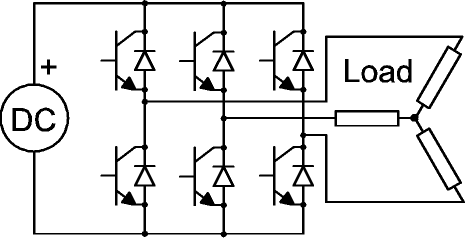
\includegraphics[height=4cm]{inv-tri.png}
            \caption{Inversor trifásico.}
            \label{fig:inv-tri}
         \end{subfigure}
      \caption{Inversores citados.}
      \label{fig:inv-esquematicos}
   \end{figure}

%=====================================================

\section{Sistemas de armazenamento de energia}

   Recentemente, a demanda de energia elétrica se tornou mais imprevisível, além disso, fontes renováveis são em sua maioria intermitentes, como a geração eólica e fotovoltaica. Sistemas de armazenamento de energia vêm para facilitar a integração dos sistemas, melhorar a estabilidade, confiabilidade, qualidade e eficiência da energia, provendo uma distribuição robusta e resiliente \cite{Zob18}.

   \subsection{Tecnologias de sistemas de armazenamento de energia}

      Várias tecnologias de armazenamento de energia vêm sendo testadas para possibilitar uma maior flexibilidade nos seus sistemas. O uso de cada uma dessas tecnologias, tem suas especificidades, variando o tempo de resposta, capacidade, dentre outros parâmetros. Na figura abaixo podemos comparar as características de potência e energia de cada tecnologia de armazenamento. Interessante é observar que baterias de íons de lítio ocupam o meio do gráfico, sendo um equilíbrio entre alta potência e energia.

      \begin{figure}[!htb]
         \centering
         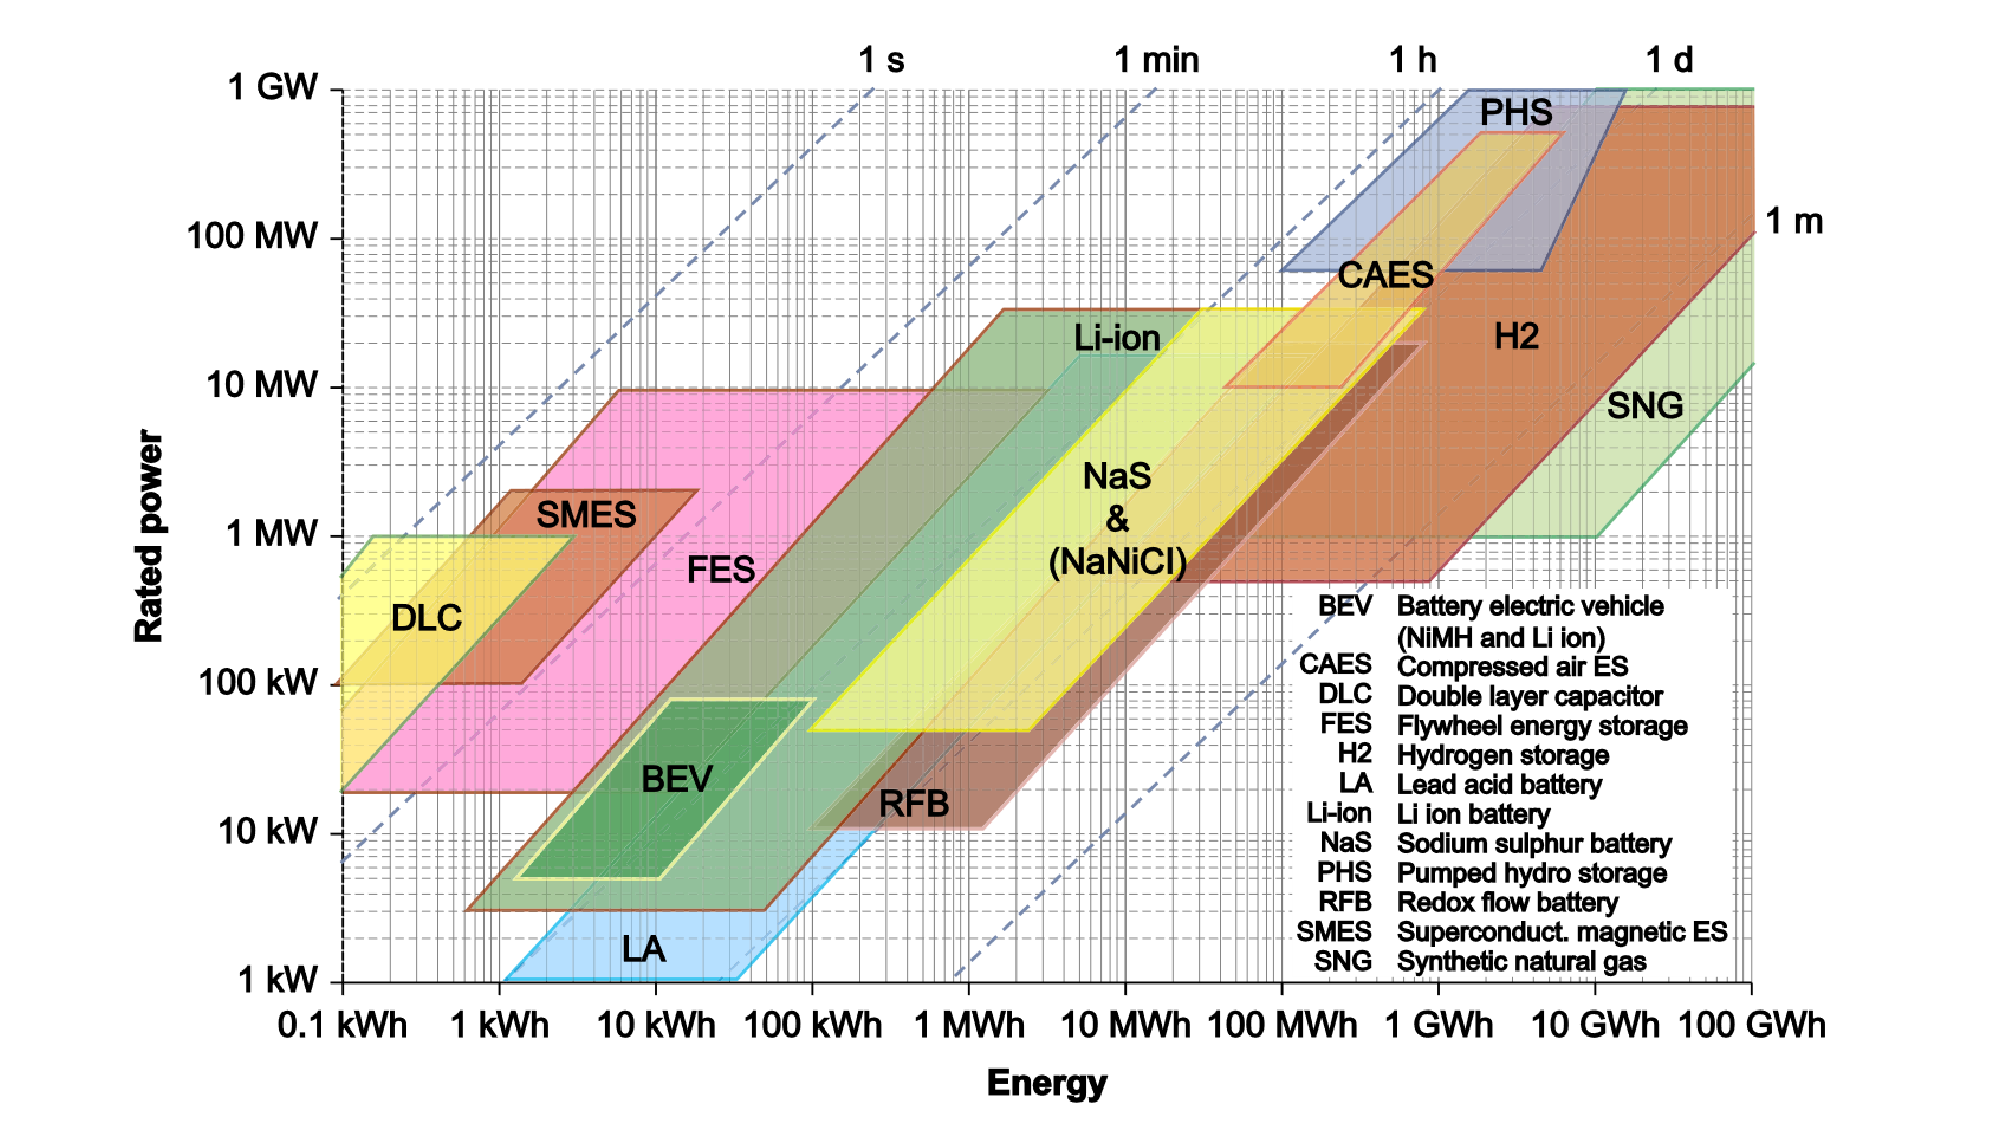
\includegraphics[width=\linewidth]{ess-ragone.pdf}
         \caption{Comparação dos parâmetros de potência e energia de diferentes sistemas de armazenamento de energia.}
         \label{fig:ess-ragone}
      \end{figure}

   \subsection{Baterias}

      Baterias normalmente são consideradas como uma invenção recente, mas foram a partir delas que surgiram os primeiros estudos no campo da eletricidade. Em 1799, Alessandro Volta (1745–1827) publicou suas descobertas ao desenvolver o que iria ser conhecido posteriormente como pilha de volta, sendo essa reconhecida como a primeira célula eletroquímica usada para o armazenamento de energia elétrica. Posteriormente, em 1859, Gaston Planté (1834–1889) desenvolve o que é considerada a primeira bateria recarregável moderna: a bateria de chumbo ácido. Esta é composta de chapas de chumbo usadas como anodo e catodo, banhadas em ácido sulfúrico, o eletrólito. Desde então, essa tecnologia vem sendo melhorada por vários pesquisadores e laboratórios ao redor do mundo, sendo hoje em dia a tecnologia com maior oferta e menor custo no mercado de armazenamento de energia em baterias \cite{War15}.

      Um outro tipo de bateria recarregável muito conhecido é a bateria de níquel cádmio (NiCd). Esta foi desenvolvida em 1899 por Ernst Waldemar Jungner (1869–1924), mas apenas por volta de 1950 se tornou comercialmente disponível. Ela se popularizou muito com o aumento do consumo de dispositivos eletrônicos portáteis, sendo a única disponível até os anos 1980. Essas baterias apresentam o efeito memória e uma menor vida útil quando comparada com outros tipos de baterias, além de serem ambientalmente danosas. Foram substituídas em sua maior parte por baterias de níquel-hidreto metálico (NiMH), que têm características muito parecidas e um impacto ambiental reduzido.

      Incentivado pelo mercado crescente de dispositivos portáteis a partir dos anos 1980, já comentado acima, inúmeras pesquisas foram desenvolvidas na tentativa de viabilizar células de íons de lítio, até então apenas teóricas. Em 1991 a Sony começa a comercialização dos primeiros dispositivos portáteis com esse tipo de tecnologia, que possui inúmeras vantagens: maior densidade de potência e energia, baixa auto descarga e não possuir o efeito memória \cite{War15}. Para resumir as características comentadas acima e trazer mais alguns detalhes, foi feita a tabela \ref{tab:bat-tecnologias} abaixo.

      \begin{table}[!htp]
         \centering
         \caption{Comparativo entre diferentes tecnologias de baterias \cite{War15}.}
         \label{tab:bat-tecnologias}
         \begin{tabular}{l m{1.9cm} m{1.9cm} m{2.2cm} m{2.2cm}}
            \hline
            \multicolumn{1}{c}{}                   & Chumbo ácido    & Níquel cádmio   & Níquel metal hidreto  & Íons de lítio\\
            \hline
            Descritor da química do catodo         & PbA/LAB         & NiCd            & NiMh                  & LCO          \\
            Energia específica (Wh/kg)             & 30-40           & 40-60           & 30-80                 & 120-150      \\
            Densidade de energia (Wh/L)            & 60-70           & 50-150          & 140-300               & 250-450      \\
            Potência específica (W/kg)             & 60-180          & 150             & 250-1000              & 600          \\
            Densidade de potência (W/L)            & 100             & 210             & 400                   & 1200-3000    \\
            Tensão nominal (V)                     & 2,0             & 1,2             & 1,2                   & 3,6-3,8      \\
            Ciclos                                 & 300-800         & 1000-2000       & 500-1500              & >700         \\
            Auto descarga (\% por mês)             & 3-5             & 20              & 30                    & 1-5          \\
            Temperatura de operação ($^{\circ}$C)  & -20 a 60        & -40 a 60        & -20 a 60              & -20 a 60     \\
            \hline
         \end{tabular}
      \end{table}
      
   \subsection{Baterias de íons de lítio}
      \subsubsection{Funcionamento}
         Baterias são dispositivos eletroquímicos, quando olhados apenas com o olhar de engenharia elétrica é comum classificar a célula de bateria como uma caixa fechada e indivisível com propriedades normalmente apenas empíricas. Mas é importante que se tenha uma visão química por diversos motivos: a segurança do sistema é dependente da estabilidade térmica interna dos componentes das células, diferentes componentes químicos utilizados nas células podem resultar em características elétricas distintas e por consequência um circuito equivalente diferente na modelagem. 

         Na figura \ref{fig:liion-funcionamento} pode-se ver uma ilustração do funcionamento de uma célula de íons de lítio no processo de descarga. É chamado de ânodo o eletrodo com o menor potencial da reação, o polo negativo, e de cátodo o polo positivo. Em células de íons de lítio, o ânodo é de algum material carbônico e o material do cátodo varia conforme o tipo da célula. Entre os eletrodos se encontra o eletrólito e o separador: o eletrólito tem por função conduzir os componentes químicos entre os eletrodos e o separador impede que elétrons passem de um lado para o outro por dentro da célula, permitindo apenas a passagem dos íons, que são átomos de lítio com carga positiva ou negativa. Conectado nos eletrodos estão os coletores de corrente, esses têm por função conduzir os elétrons para o exterior da célula e são de material metálico.

         \begin{figure}[!htb]
            \centering
            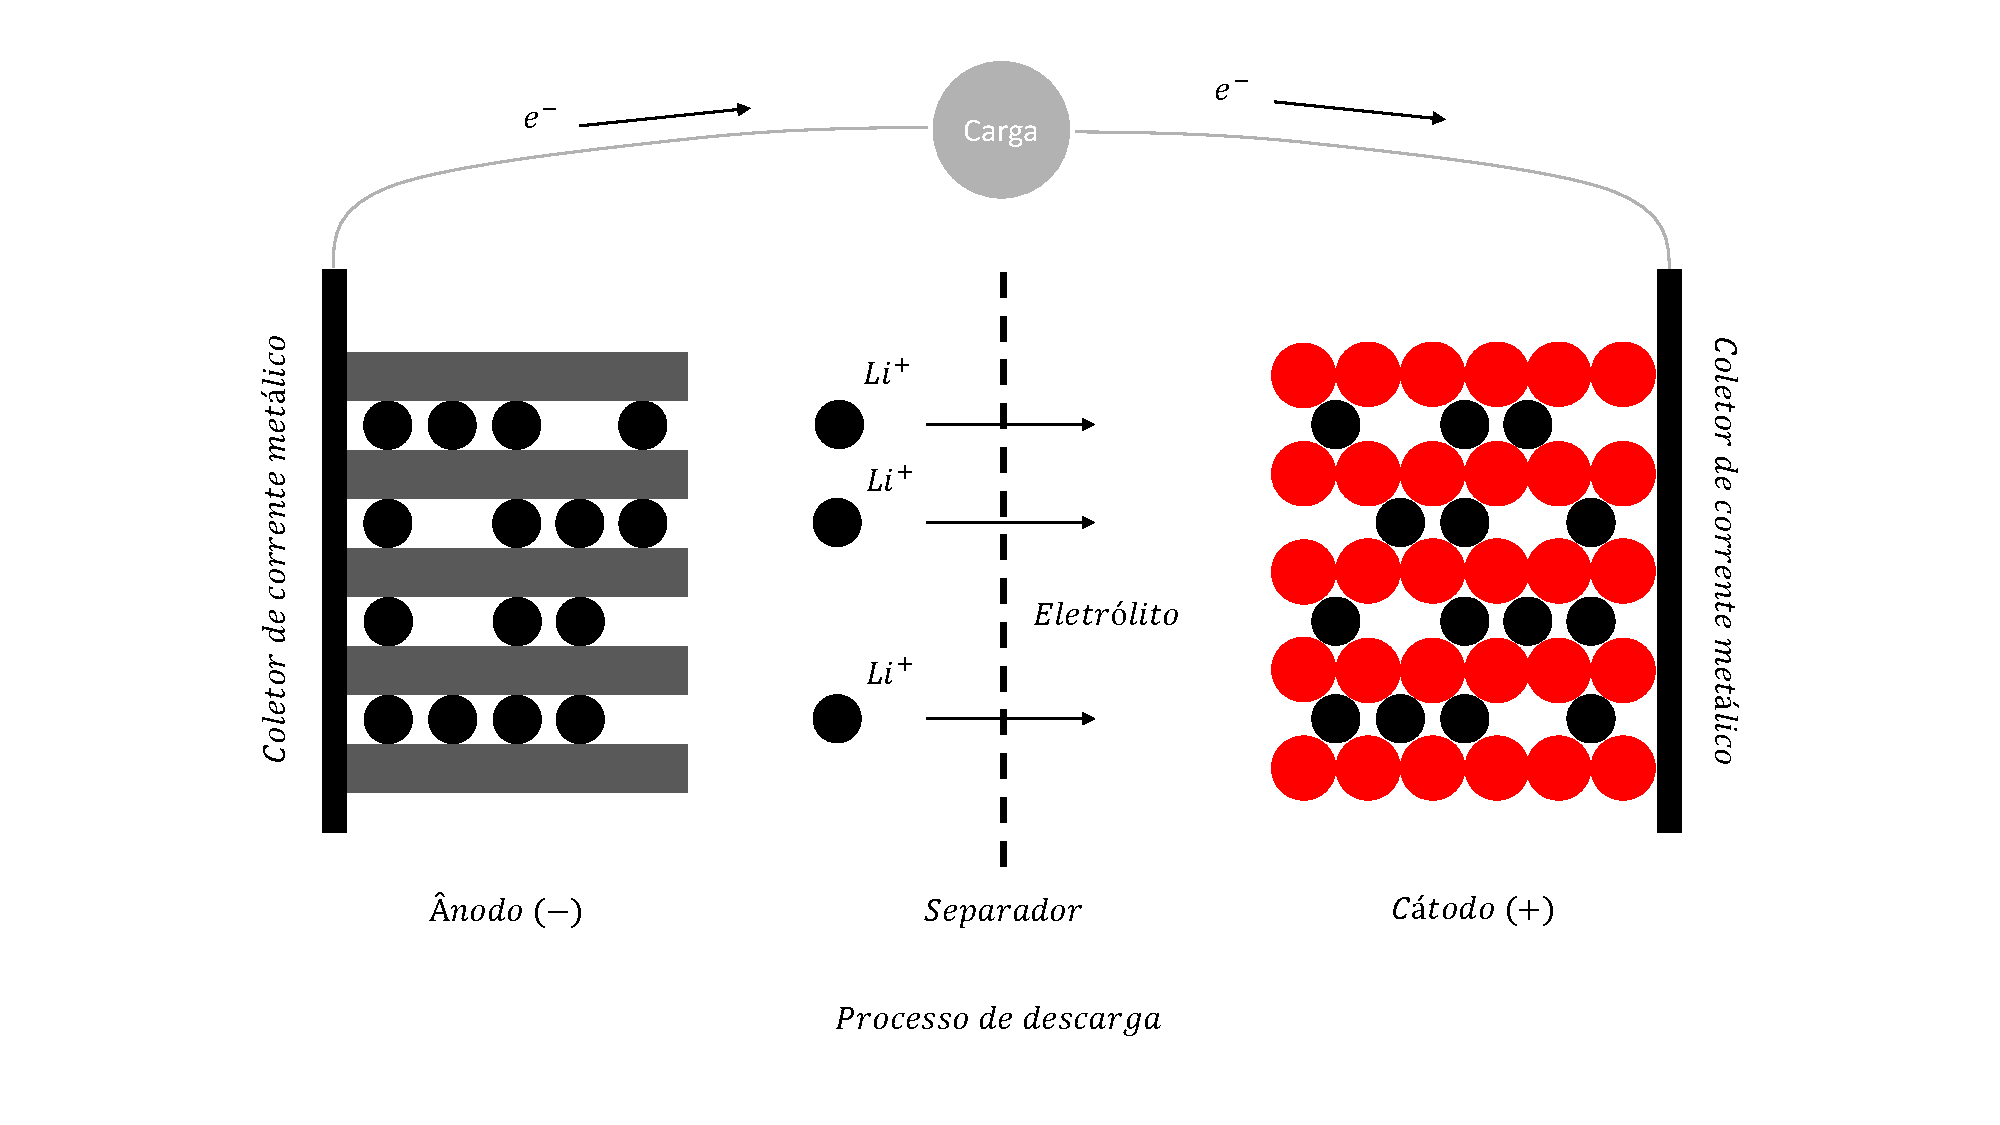
\includegraphics[width=\linewidth]{liion-funcionamento.pdf}
            \caption{Esquema de funcionamento de uma célula de íons de lítio. Adaptado de \cite{Wal18}}
            \label{fig:liion-funcionamento}
         \end{figure}
   
         A bateria ganha sua capacidade de armazenar energia elétrica quando os átomos de íons de lítio se intercalam no ânodo ou cátodo durante a descarga e a carga. Na figura \ref{fig:liion-funcionamento} está representado o processo de descarga de uma célula, sendo que na carga apenas os sentidos dos íons de lítio e da corrente se invertem.

         Baterias de íons de lítio não são apenas um tipo de bateria com uma composição química, mas sim um conjunto de diferentes tipos. Isso se dá, normalmente, pela variação dos componentes do cátodo. Tipos muito comuns são o NCA (Lítio Níquel Cobalto Alumínio) e o NMC (Lítio Níquel Manganês Cobalto) que apresentam as maiores densidades de energia. Mas é possível encontrar outros tipos com propósitos mais específicos, como LTO (Titanato de Lítio), que é muito segura e tem uma alta densidade de potência.

      \subsubsection{Formatos}
         Assim como a química varia entre diferentes células de baterias de íons de lítio, há uma variedade de formatos. Entre os principais formatos comercializados atualmente estão: células prismáticas, \textit{pouch} e cilíndricas. 

         As vantagens da célula cilíndrica incluem uma maior facilidade de fabricação e uso, resistência mecânica e um controle térmico facilitado. Um dos tamanhos mais comuns de bateria cilíndrica é o padrão 18650, medindo 18 mm de diâmetro e 65 mm de comprimento, mas variantes, como 21700 ou 20650, vêm se tornando cada vez mais comuns.

      \subsubsection{Segurança}
         Se tornou comum nos últimos anos vermos notícias de falhas em baterias de íons de lítio que causam todo tipo de problema, desde voos cancelados quando smartphones pegam fogo dentro da cabine até robô protótipo da NASA (Administração Nacional da Aeronáutica e Espaço dos Estados Unidos) sendo destruído após explosão das baterias. Assim, é necessário que tomemos todos os cuidados ao projetar um acumulador, entendendo o que leva as células à falha e prevendo formas evitar isso.

         Essa preocupação com a segurança vem de um efeito chamado \textit{Thermal Runaway} que acontece em células de íons de lítio. Que é basicamente uma reação em cadeia de aquecimento que gera um \textit{feedback} positivo até sua destruição. Em elevadas temperaturas uma decomposição exotérmica dos componentes internos da bateria começa, quando o calor gerado nessa reação é maior que a capacidade da célula de dissipar se inicia o auto aquecimento. A taxa de decomposição aumenta conforme a temperatura, seguindo a equação de Arrhenius. Eventualmente, a estabilidade da célula é perdida, o que leva à ruptura da mesma, liberando o restante da energia eletroquímica armazenada na célula. A propagação é uma reação em cadeia quando a energia liberada de uma célula se espalha para as células adjacentes, fazendo com que elas aqueçam o suficiente para iniciar a decomposição exotérmica interna \cite{Wal18}.

         \begin{figure}[!htb]
            \centering
            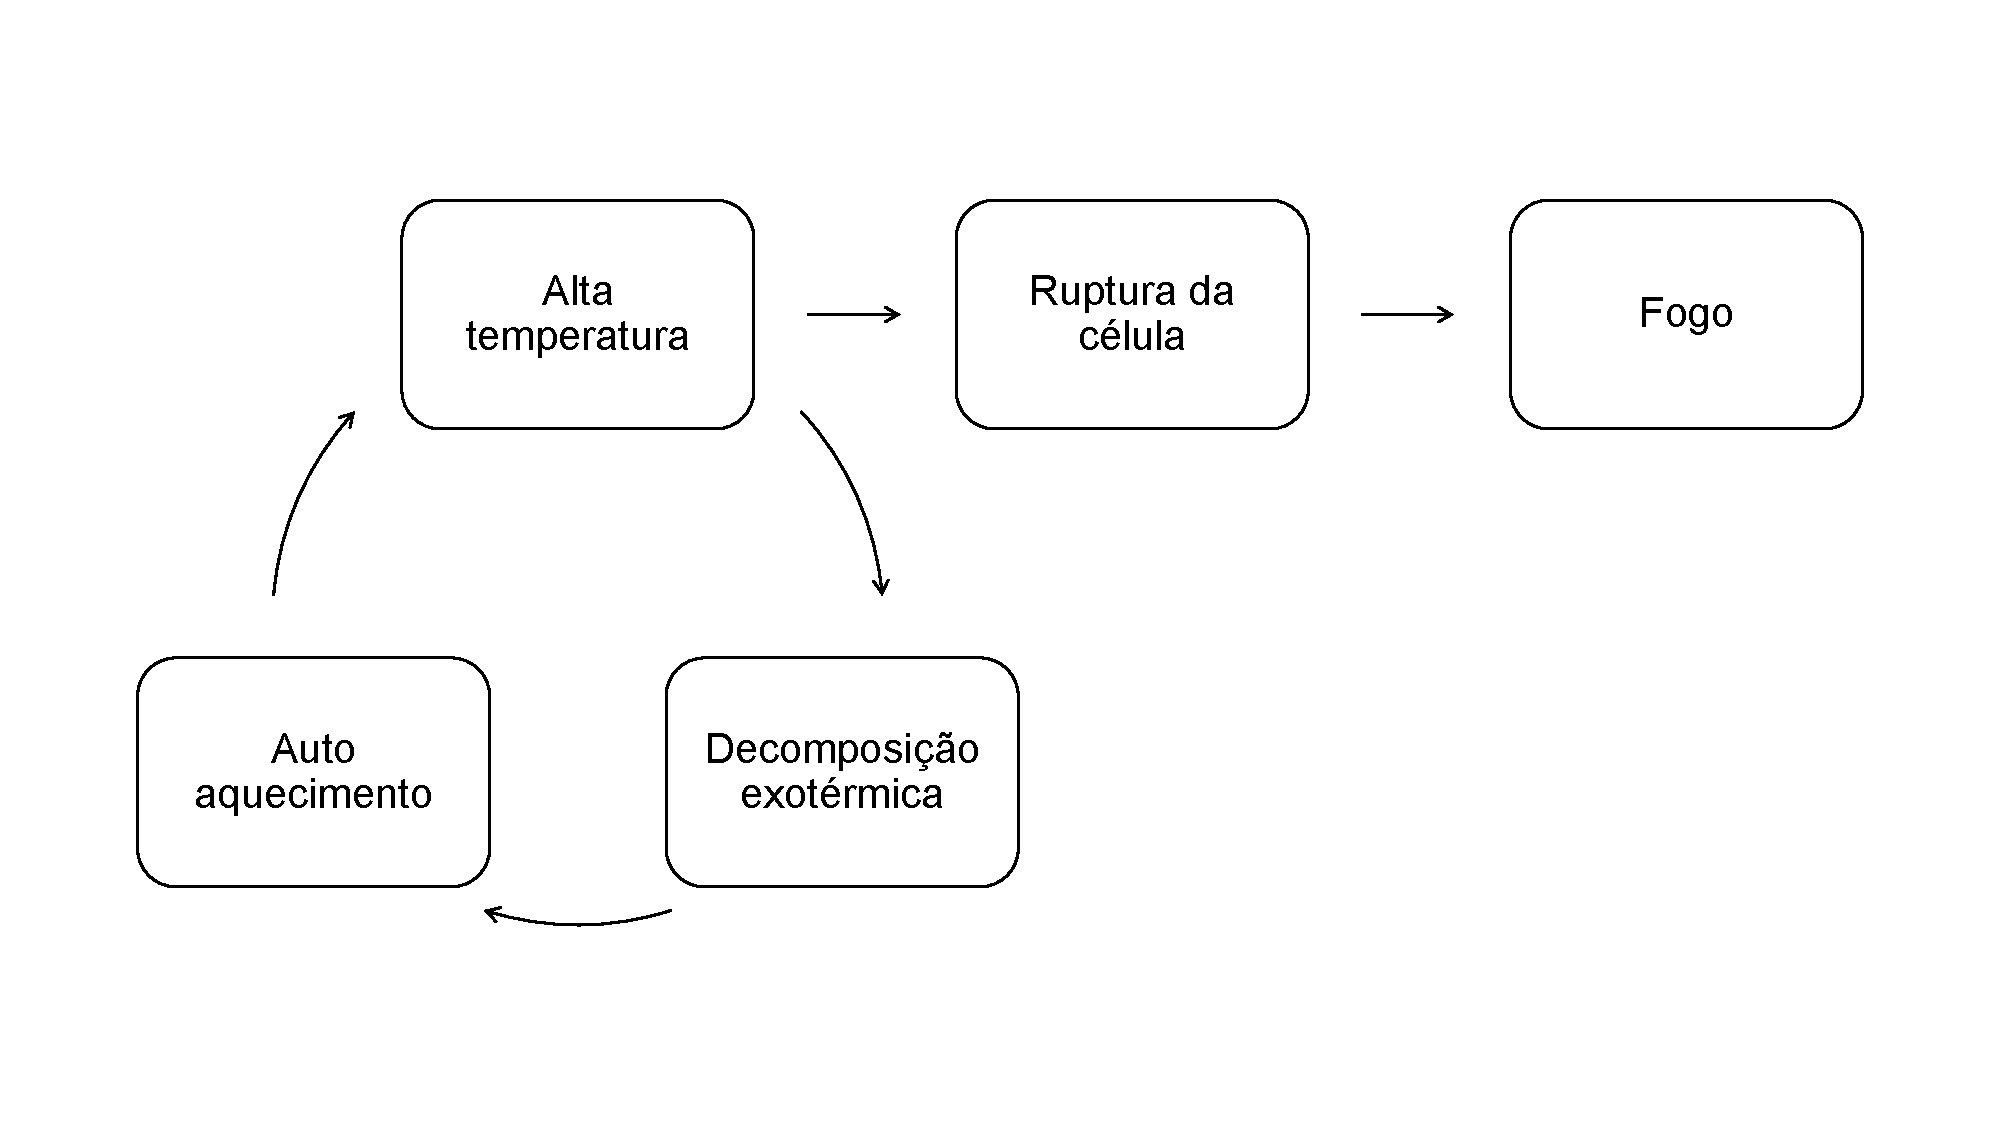
\includegraphics[width=12cm]{liion-therm-runaway.pdf}
            \caption{Esquema do funcionamento de um \textit{Thermal Runaway}}
            \label{fig:liion-therm-runaway.pdf}
         \end{figure}

         Como mostrado, essa reação se inicia com uma alta temperatura e pode ter resultados catastróficos. Mas vários motivos podem causar esse aquecimento da célula, sendo eles: a falha térmica, que seria devido à elevadas temperaturas externas; a falha mecânica, quando a célula sofre penetração ou é dobrada; curto circuito interno, normalmente causado por falhas de manufatura das células; curto circuito externo; e abuso eletroquímico, que inclui sobrecarga e sobredescarga da célula. Cada um desses motivos deve ser investigado e cuidado deve ser tomado ao projetar sistemas de mitigação de cada uma dessas falhas.

         No projeto de um acumulador é incluído um dispositivo de gerenciamento e monitoramento das células, conhecido como BMS. Esse tem por função medir a tensão, temperatura e corrente, além de ter a capacidade de controlar os dispositivos que usam a energia da bateria e em últimos casos desconectar o sistema. Um projeto mecânico sólido e bem feito do container pode prevenir falhas mecânicas, e o uso de fusíveis impedir curto-circuito.		% fundamentação teórica
\chapter{Materiais e métodos}
\label{cap:exemplos}

% figuras estão no subdiretório "figuras/" dentro deste capítulo
\graphicspath{{\currfiledir/figuras/}}

%=====================================================

No início da fase de projetos foi definida uma estrutura de organização: uma adaptação do sistema \textit{waterfall} descrito em \cite{Ian19}). Apesar deste ter sido desenvolvido para projetos de software, é comum a adaptação e utilização em outros tipos de projeto. Esse sistema se forma ao alinhar, uma após a outra, as tarefas do desenvolvimento de um projeto, como mostrado na figura \ref{fig:metodologia}:

\begin{figure}[!htb]
    \centering
    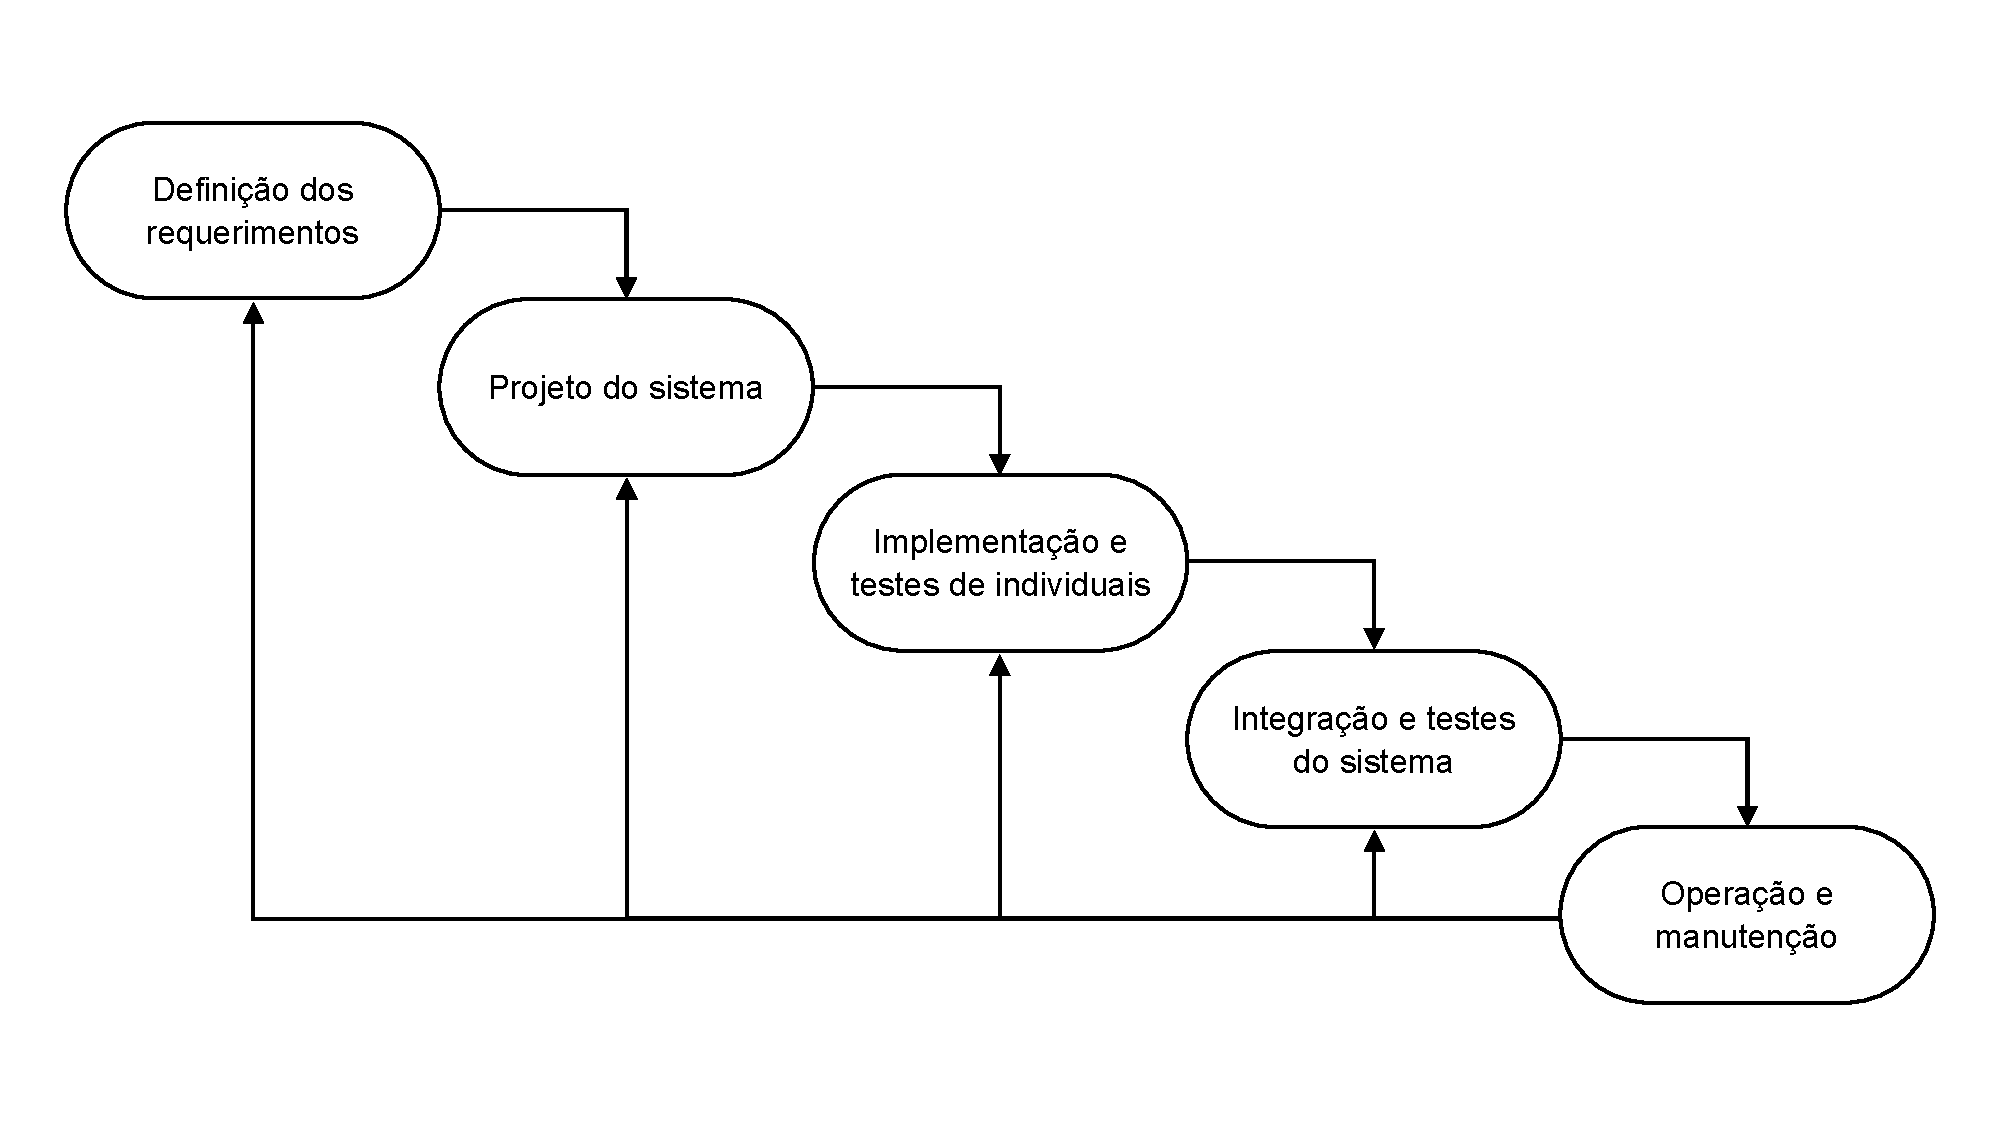
\includegraphics[width=\linewidth]{metodologia.pdf}
    \caption{Esquema das fases do projeto.}
    \label{fig:metodologia}
\end{figure}

Dentro de cada uma dessas fases de projeto diferentes atividades e documentos são desenvolvidos. A começar pela primeira etapa: definição dos requerimentos. Aqui, o processo se inicia ao criar uma lista de requerimentos, buscando responder o que é esperado do sistema projetado. A partir disso é feito um detalhamento na etapa de especificação dos requerimentos, tentando aplicar valores bem definidos como limite. Por último é feita uma validação dos requerimentos. Essa etapa gera o documento de requerimentos, que inclui a descrição dos sistemas e os requerimentos dos usuários e dos sistemas. Esse documento é usado de guia para todo o restante do projeto e a partir dele devem ser justificadas as decisões de projeto.

A próxima etapa é o desenvolvimento do projeto do sistema em si. Esse se inicia e é baseado nos documentos de entrada: o documento de requerimentos e informações dos dispositivos utilizados. A partir daí é desenvolvido o projeto de arquitetura do sistema, onde é identificada a estrutura geral do projeto e seus principais componentes, com módulos ou submódulos, como esses são distribuídos e como se relacionam. De forma mais especifica, esse relacionamento entre os módulos do é desenvolvido no projeto da interface, que descreve o relacionamento entre os componentes e com o mundo externo. E por último, é desenvolvido o projeto específico dos componentes, especificando de forma exata para que seja possível a manufatura a partir dessas especificações. Cada uma dessas atividades gera seu respectivo documento, que é utilizado como referência para cada etapa seguinte.

Com todo o projeto finalizado são desenvolvidos os testes, a começar por testes dos componentes de forma individual, após isso um teste de integração e por último, o teste completo do sistema, onde todos os requerimentos são observados e verificados se estão sendo atendidos de forma aceitável pelo sistema. Toda a documentação de planejamento de testes e os resultados deve ser desenvolvida e após isso o sistema está apto para ser utilizado pelo usuário.

Para o desenvolvimento do projeto que esse documento descreve, o sistema de armazenamento de energia foi dividido em diversos subsistemas, cada um com seus requerimentos e projetos específicos. Além disso, pelas diferenças que um projeto de sistema de armazenamento para mobilidade elétrica tem em relação à um sistema de armazenamento estacionário, alguns dos subsistemas que são empregados em veículos elétricos não estão presentes no sistema estacionário, sendo os subsistemas listados abaixo:

\begin{itemize}

    \item Veículo elétrico
    
    \begin{enumerate}
        \item Acumulador / Células
        \item Container
        \item Conexões
        \item Segmentos
        \item Plugs de manutenção
        \item HV Disconnect (HVD)
        \item Medidor de energia
        \item Fusíveis
        \item Fusível principal
        \item Relés de isolamento do acumulador (AIRs)
        \item Indicador LED do acumulador
        \item Circuito de pré-carga
        \item Circuito de descarga
        \item Circuito Shutdown
        \item Placas de circuito impresso (PCBs)
        \item Sistema de gerenciamento do acumulador (AMS)
        \item Dispositivo de monitoramento do isolamento (IMD)
        \item Carregador
        \item Circuito Shutdown do carregador
    \end{enumerate}

    \item Microrrede
    
    \begin{enumerate}
        \item Acumulador / Células
        \item Container
        \item Conexões
        \item Plugs de manutenção
        \item Fusíveis
        \item Fusível principal
        \item Relés de isolamento do acumulador (AIRs)
        \item Circuito de pré-carga
        \item Circuito de descarga
        \item Circuito Shutdown
        \item Placas de circuito impresso (PCBs)
        \item Sistema de gerenciamento do acumulador (AMS)
    \end{enumerate}
    
\end{itemize}





			% materiais e métodos
\chapter{Resultados e Discussão}
\label{cap:exemplos}

% figuras estão no subdiretório "figuras/" dentro deste capítulo
\graphicspath{{\currfiledir/figuras/}}

%=====================================================

\section{Acumulador / Células}

    É o conjunto de todas as células de bateria ou supercapacitores que armazenam energia elétrica para ser usada no sistema de tração (\textit{Tractive System – TS}), no veículo elétrico, ou no sistema de alta tensão (\textit{High Voltage System – HVS}), na microrrede. Não existem muitos requerimentos nessa parte, principalmente no sistema da microrrede. Já no veículo elétrico, a tensão máxima é limitada em 600 V.

    A escolha do modelo de célula a ser utilizada se iniciou com uma pesquisa de fabricantes, sendo LG, Samsung e Panasonic/Sanyo as mais conhecidas e disponíveis. Apenas células cilíndricas são usadas, sua preferência é justificada pelo uso facilitado, a não necessidade de um container com controle de pressão, a presença de dispositivos de proteção internos, além da experiência prévia no uso de células cilíndricas em projetos anteriores. Uma lista das melhores células dessas fabricantes foi feita.

    Características do \textit{datasheet} foram observadas ao montar o gráfico da figura \ref{fig:ragone-celulas}, comparando a energia específica e potência específica das células. É possível ver uma clara distinção entre células de alta potência e células de alta energia, sendo as de alta potência na parte mais à direita do gráfico e as de alta energia na parte superior.

    \begin{figure}[!htb]
        \centering
        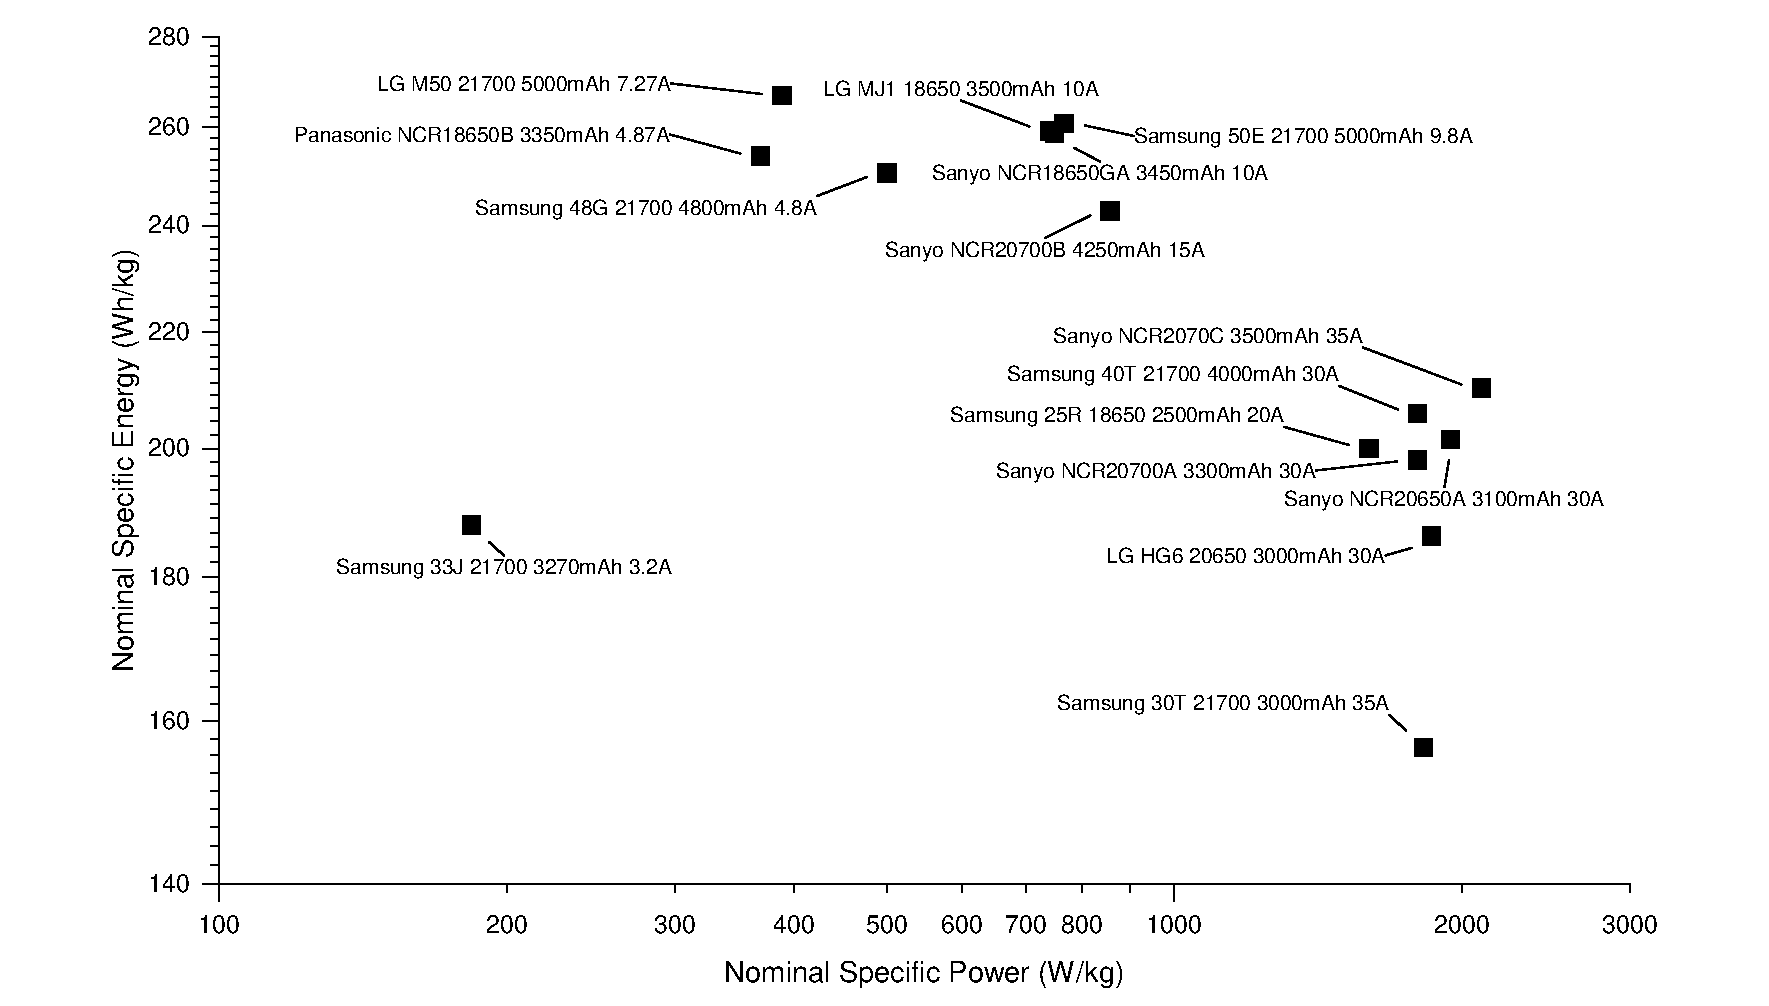
\includegraphics[width=\linewidth]{ragone-celulas.pdf}
        \caption{Comparação de dados do datasheet dos modelos de células analisados.}
        \label{fig:ragone-celulas}
    \end{figure}

    Desses modelos apresentados acima, os 11 mais promissores foram adquiridos para o desenvolvimento dos testes. Estes foram feitos seguindo os principais padrões internacionais (como a IEC 62660-1:2010). 

    Inicialmente é realizado um teste de pré-condicionamento (\textit{Preconditioning Test}) para verificar se a capacidade da célula se mantém constante em testes seguidos, além de preparar a célula para os testes seguintes. Após isso é realizado o ciclo padrão (\textit{Standard Cycle}) com o objetivo de verificar a capacidade nominal da célula. O teste de capacidade (\textit{Capacity Test}) é realizado, em seguida, para se obter o valor da capacidade em função da corrente de teste (tabela \ref{tab:40T-testeresultados-cap} e figura \ref{fig:40T-testegraf-cap}). Após isso, é feito o teste de ciclo de baixa corrente (\textit{Low C-rate Cycle}), que tem por objetivo obter o valor da tensão de circuito aberto em relação ao estado de carga (figura \ref{fig:40T-testegraf-ocv}). Por último, o teste de impedância eletroquímica (\textit{Electrochemical Impedance Spectroscopy – EIS}), que tem por objetivo monitorar a relação entre a impedância da célula e seu estado de carga, durante os ciclos de carga e descarga (figura \ref{fig:40T-testegrafs-imp}).

    \begin{table}[!htp]
        \centering
        \caption{Resultados do teste da capacidade da célula Samsung 40T.}
        \label{tab:40T-testeresultados-cap}
        \begin{tabular}{lccc}
           \hline
           \multicolumn{1}{c}{}& Tensão média & Carga & Energia \\
           \hline
           0,2C & 3,646 V & 3,970 Ah & 14,483 Wh \\
           0,5C & 3,634 V & 3,891 Ah & 14,145 Wh \\
           1C   & 3,599 V & 3,842 Ah & 13,833 Wh \\
           5C   & 3,441 V & 3,874 Ah & 13,216 Wh \\
           \hline
        \end{tabular}
    \end{table}
    
    \begin{figure}[!htb]
    \centering
        \begin{subfigure}{0.48\linewidth}
            \centering
            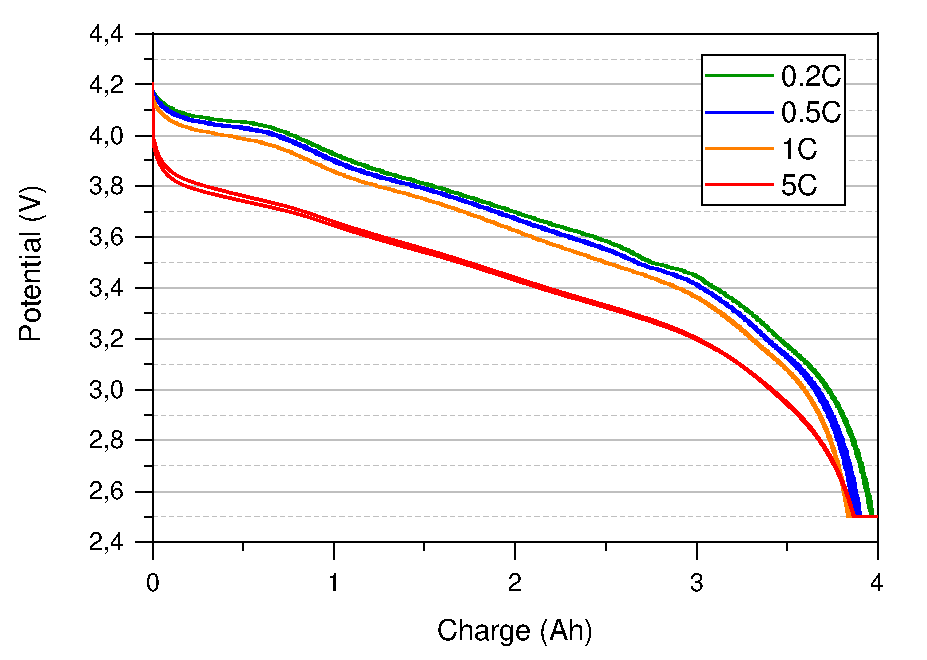
\includegraphics[width=\linewidth]{40T-testegraf-cap.pdf}
            \caption{Capacidade em relação a carga.}
            \label{fig:40T-testegraf-cap}
        \end{subfigure}
        \hspace*{\fill}
        \begin{subfigure}{0.48\linewidth}
            \centering
            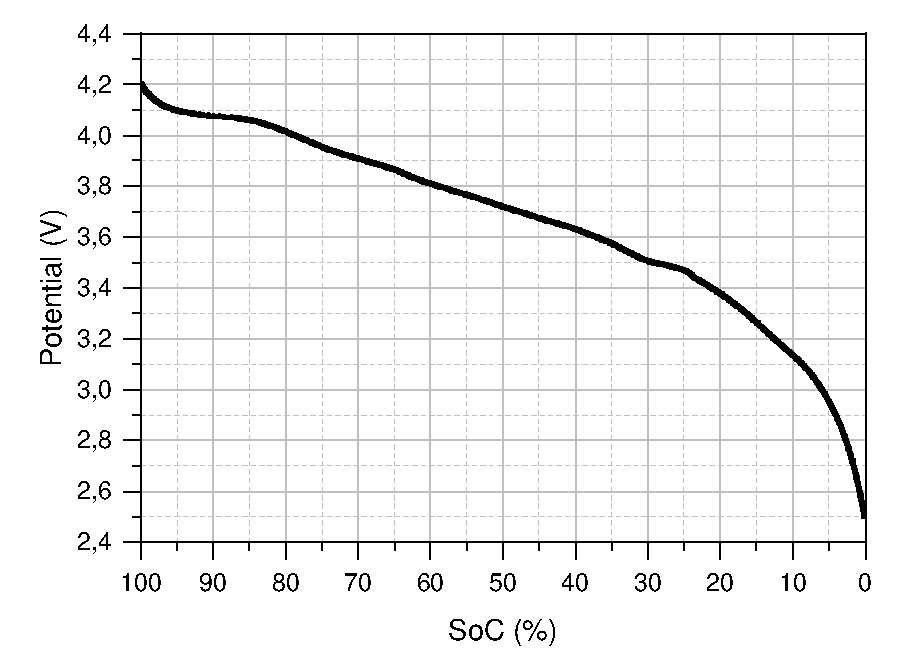
\includegraphics[width=\linewidth]{40T-testegraf-ocv.pdf}
            \caption{Tensão de circuito aberto em relação ao estado de carga (SoC).}
            \label{fig:40T-testegraf-ocv}
        \end{subfigure}
    \caption{Graficos dos testes da célula Samsung 40T.}
    \label{fig:40T-testegrafs-cap}
    \end{figure}
     
    \begin{figure}[!htb]
        \centering
            \begin{subfigure}{0.48\linewidth}
                \centering
                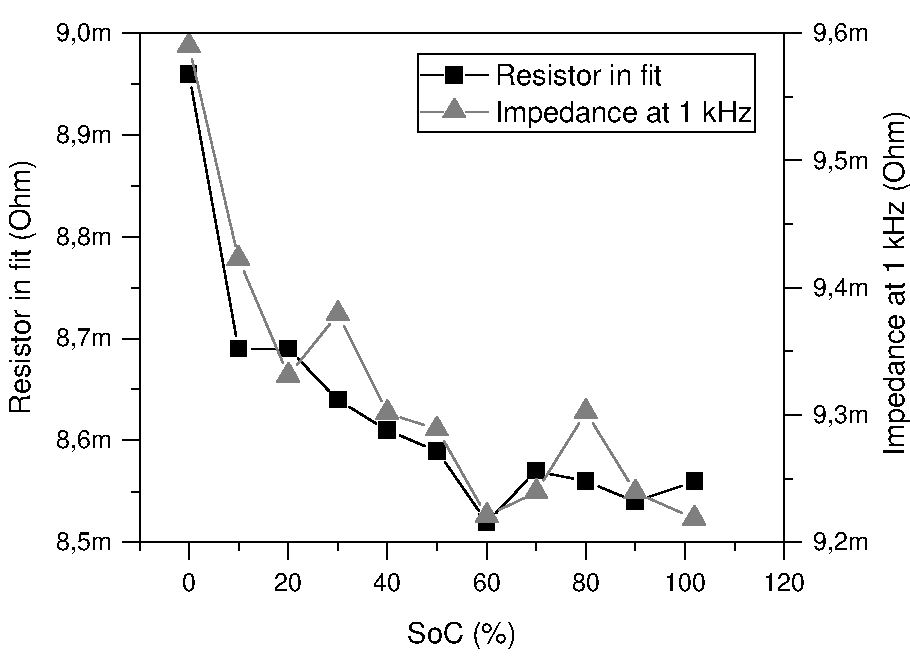
\includegraphics[width=\linewidth]{40T-testegraf-imc.pdf}
                \caption{Carga.}
                \label{fig:40T-testegraf-imc}
            \end{subfigure}
            \hspace*{\fill}
            \begin{subfigure}{0.48\linewidth}
                \centering
                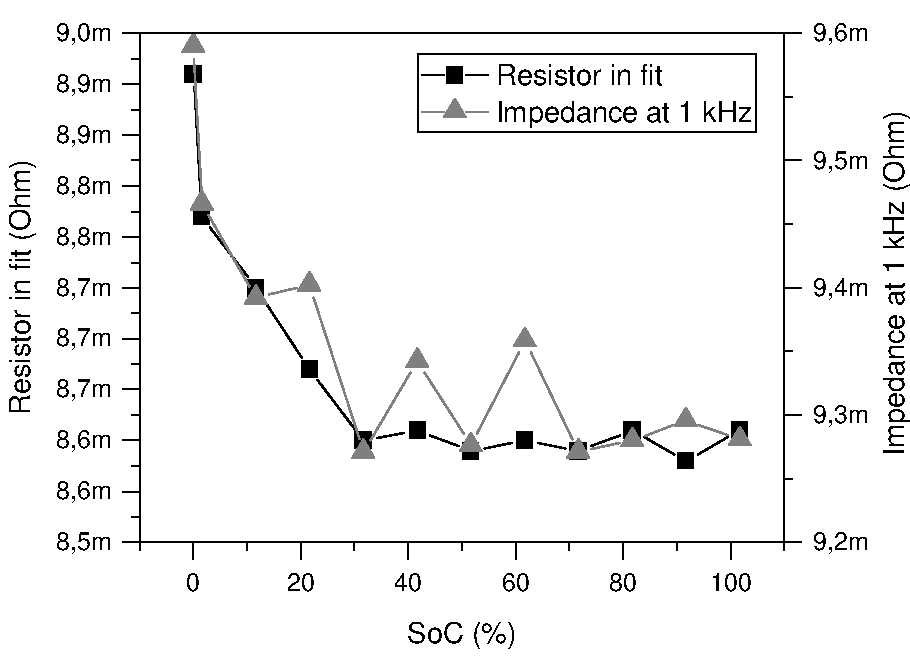
\includegraphics[width=\linewidth]{40T-testegraf-imd.pdf}
                \caption{Descarga.}
                \label{fig:40T-testegraf-imd}
            \end{subfigure}
        \caption{Graficos dos testes de impedância em relação ao estado de carga (SoC) da célula Samsung 40T.}
        \label{fig:40T-testegrafs-imp}
    \end{figure}

    Apesar de todas as células de testes terem sido adquiridas, não foi possível realizar todos os testes previstos em razão da pandemia de COVID-19. Sendo que foi possível a coleta de dados de apenas uma unidade da célula Samsung 40T. Desta forma, infelizmente, não foi possível que houvessem dados reais de teste para o embasamento da escolha das células, assim, serão usados apenas dados do datasheet. Apesar de não ter sido possível a comparação com dados dos demais modelos de célula, os dados abaixo da célula Samsung 40T foram usados para a simulações da célula.

    Com os dados de datasheet já comparados anteriormente, foi observado que a célula Samsung 40T é a que apresenta o melhor desempenho de potência com uma energia satisfatória e a Samsung 50E apresenta o melhor desempenho de energia com uma potência satisfatória, por isso, foram escolhidas para serem utilizadas nos dois acumuladores sendo desenvolvidos: 40T para o veículo elétrico e 50E para a microrrede. 

    Após as células terem sido escolhidas foi feito o dimensionamento do acumulador, ou seja, a quantidade de células em série e paralelo. Inicialmente os valores de referência foram definidos, para a tensão, energia e corrente (tabela \ref{tab:acc-desejado}). As tensões máximas foram definidas para estarem próximas dos máximos permitidos pelos sistemas nas quais elas seriam conectadas: 600 V nominal e 800 V máximo para o conversor CC-CC da microrrede, 550 V máximo para o motor do veículo elétrico. Além disso levando em consideração a segurança de quem for realizar manutenção e operação dos sistemas, a tensão da microrrede será limitada em 600 V. A tensão máxima do veículo foi também limitada abaixo de 500 V para que os componentes de potência utilizados em sistemas de segurança sejam mais simples e por consequência mais leves. A corrente máxima, no veículo, de 170 A foi definida para que seja possível ter um bom desempenho de potência, para garantir uma aceleração rápida em qualquer circunstância. A energia total do sistema da microrrede de 20 kWh foi um requerimento apresentado pelo sistema e previamente calculado em outros estudos. A energia do veículo elétrico, de 6kWh, foi estimada para que seja possível andar por volta de 20 km com uma carga, que seria o equivalente à prova mais longa da competição. Para isso foram feitas simulações do desempenho do sistema de tração em conjunto com o restante do carro.

    \begin{table}[!htp]
        \centering
        \caption{Valores desejados para o dimensionamento dos sistemas.}
        \label{tab:acc-desejado}
        \begin{tabular}{lcc}
            \hline
            Sistema                                      & Microrrede    & Veículo elétrico  \\
            Energia [Wh]                                 & 20000 Wh      & 6000 Wh           \\
            Corrente máxima [A]                          & 120,00 A      & 170,00 A          \\
            Tensão máxima desejada [V]                   & 600 V         & 480 V             \\
            Tensão máxima do sistema conectado [V]       & 800 V         & 550 V             \\
            Tensão máxima permitida (regulamento) [V]    & --            & 600 V             \\
            \hline
        \end{tabular}
    \end{table}

    Com esses dados foi possível calcular a quantidade de células necessária. Inicialmente calculando a quantidade de células em série, apenas dividindo a tensão máxima desejada pela tensão máxima de uma célula. Esses valores foram, então, arredondados para melhor encaixarem na montagem final. Após isso, a quantidade de células em paralelo desejada foi calculada de duas formas: a partir da corrente (potência) e a partir da energia. Pode-se ver que em ambos os casos esses dois valores acabam sendo parecidos, refletindo a boa escolha da célula para as necessidades do sistema. Novamente, foi arredondado o valor das células em paralelo. Na tabela \ref{tab:acc-projeto} é possível ver todas as características calculadas do acumulador.

    \begin{table}[!htp]
        \centering
        \caption{Características do acumulador.}
        \label{tab:acc-projeto}
        \begin{tabular}{lcc}
            \hline
            Sistema                                         & Microrrede    & Veículo elétrico  \\
            Fabricante                                      & Samsung       & Samsung           \\
            Modelo                                          & INR21700-50E  & INR21700-40T      \\
            Células em série (calculado)                    & 142,86        & 114,29            \\
            Células em série (arredondado)                  & 144           & 115               \\
            Células em paralelo (calculado para potência)   & 8,16          & 3,78              \\
            Células em paralelo (calculado para energia)    & 7,72          & 3,62              \\
            Células em paralelo (arredondado)               & 8             & 4                 \\
            Número total de células                         & 1152          & 460               \\
            Capacidade nominal [mAh]                        & 40 Ah         & 16 Ah             \\
            Corrente nominal de descarga contínua [A]       & 7,84 A        & 3,20 A            \\
            Corrente máxima de descarga contínua [A]        & 117,60 A      & 180,00 A          \\
            Corrente nominal de carga contínua [A]          & 19,60 A       & 8,00 A            \\
            Corrente máxima de carga contínua [A]           & 39,20 A       & 24,00 A           \\
            Corrente de fim de carga (Cut-off) [mA]         & 784 mA        & 400 mA            \\
            Corrente de curto circuito [A]                  & 822,86 A      & 1200,00 A         \\
            Tensão máxima [V]                               & 604,80 V      & 483,00 V          \\
            Tensão nominal [V]                              & 518,40 V      & 414,00 V          \\
            Tensão mínima [V]                               & 360,00 V      & 287,50 V          \\
            Impedância AC máxima em 1kHz [m$\Omega$]        & 4,38 m$\Omega$& 3,00 m$\Omega$    \\
            Potência nominal [W]                            & 4,064 kW      & 1,325 kW          \\
            Potência nominal (corrente máxima) [W]          & 60,964 kW     & 74,520 kW         \\
            Potência máxima [W]                             & 71,124 kW     & 86,940 kW         \\
            Energia nominal [Wh]                            & 20736 Wh      & 6624 Wh           \\
            Volume [L]                                      & 26,2679 L     & 11,4365 L         \\
            Massa [g]                                       & 79,49 kg      & 32,20 kg          \\
            \hline
        \end{tabular}
    \end{table}

%=====================================================

\section{Segmentos}

    São subgrupos de células de bateria que podem ser isoladas entre si, de forma que atendem as especificações do item EV.4.1.2 do regulamento para Formula SAE. É um sistema somente do veículo elétrico, não se deve confundir os segmentos do veículo elétrico com os módulos do acumulador da microrrede, justamente pelas especificidades desse regulamento para o uso em veículos. É usado como forma de proteção quando manutenção do sistema HV é necessária. Além disso permite ainda uma modularidade do sistema, semelhante à função dos módulos. Têm a tensão máxima limitada em 120 V e a energia máxima limitada em 6 MJ por segmento. O acumulador do veículo elétrico foi então separado em 5 segmentos, cada um com 23 células em série e 96,6 V de tensão máxima, com a energia máxima total de 5,56 MJ. 
    
%=====================================================

\section{Container}

    O container é o invólucro de todas as células do Acumulador. Usado para proteger e isolar elas fisicamente e eletricamente de qualquer agente externo. Além disso, provém local para todos os sistemas de controle e monitoramento das células, como o Sistema de gerenciamento do acumulador (AMS), o Dispositivo de monitoramento do isolamento (IMD), os Relés de isolamento do acumulador (AIRs), Circuito de pré-carga, Circuito de descarga e outros. O container deve seguir uma série de requerimentos para ser considerado seguro, dentre eles, podemos citar o eficiente isolamento elétrico, com proteção contra entrada de água, e o uso de materiais adequados. Já na microrrede o isolamento é muito importante, mas não tanto a proteção contra água, já que será usado em ambiente interno.

    Inicialmente, no projeto mecânico do acumulador, foi feita a divisão das células em módulos. Isso tem por objetivo facilitar a manutenção e manufatura, ao dividir a montagem em partes modulares. Assim, é possível que estes módulos sejam substituídos por outros sobressalentes em pouco tempo. No acumulador da microrrede foi possível dividir todas as células em módulos de igual tamanho, 12 módulos de 12 células em série. Já no acumulador do veículo elétrico, devido às limitações impostas pela divisão em segmentos, foi necessário separar em dois tamanhos diferentes de módulo: um com 11 células em série e outro com 12 células em série, totalizando as 23 células por segmento. Ou seja, cada segmento do sistema do veículo elétrico é formado por um módulo contendo 11 células em série e outro módulo contendo 12 células em série.

    O projeto da montagem física dos módulos partiu de conceitos diferentes para cada sistema. Enquanto o projeto do sistema estacionário focou na simplicidade de operação, o projeto do sistema automotivo focou no aumento da densidade. Tiveram também suas fixações feitas a partir de materiais diferentes e com formato diferente. No sistema da microrrede um espaçamento grande entre as células foi mantido, para que não seja necessário resfriamento ativo, deixando o projeto mais simples (figura \ref{fig:cont-mod-mic}). A fixação das células foi feita com chapas de policarbonato cortadas no encaixe exato. Policarbonato foi escolhido por ser um material antichamas e isolante elétrico, além de ter uma boa disponibilidade no mercado. No projeto dos módulos para o veículo elétrico, como já mencionado, foi tentado se obter a maior densidade possível. Para isso as células foram dispostas entre si na diagonal, aproveitando o espaço que ficaria entre elas (figura \ref{fig:cont-mod-vee}). A fixação das células foi feita em impressora em 3D, utilizando filamento antichamas e isolante elétrico. Esse material proporcionou mais flexibilidade no desenvolvimento do projeto, principalmente para a otimização do espaço. O ponto negativo na diminuição do espaçamento entre as células é a perda da capacidade de dissipação de calor. Este teve que ser bem planejado, evitando que o acumulador apresente uma redução no desempenho ou ainda problemas relacionados à segurança.

    \begin{figure}[!htb]
        \centering
        \begin{subfigure}{0.48\linewidth}
            \centering
            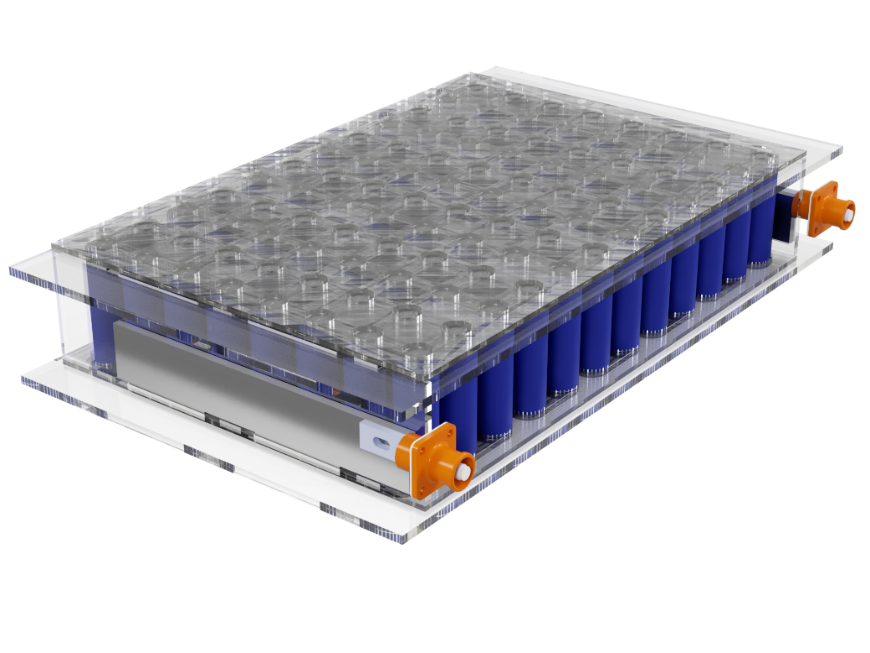
\includegraphics[height=5cm]{cont-mod-mic.png}
            \caption{Microrrede.}
            \label{fig:cont-mod-mic}
        \end{subfigure}
        %\hspace*{\fill}
        \begin{subfigure}{0.48\linewidth}
            \centering
            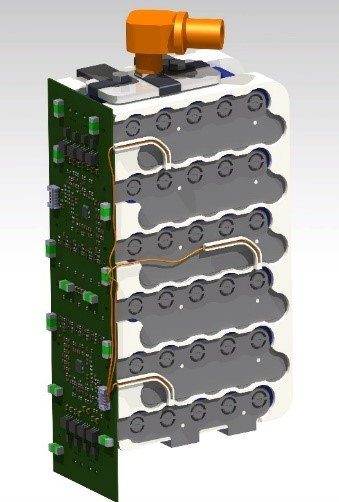
\includegraphics[height=5cm]{cont-mod-vee.jpg}
            \caption{Veículo elétrico.}
            \label{fig:cont-mod-vee}
        \end{subfigure}
        \caption{Rederização dos projetos dos módulos.}
        \label{fig:cont-mods}
    \end{figure}

    Assim como o projeto dos módulos, a montagem global dos sistemas partiu de conceitos diferentes. No sistema da microrrede o foco foi a facilidade de manutenção e instalação do sistema, assim, se optou pelo uso de racks para servidores (figura \ref{fig:cont-mod-mic}). Já o container do projeto do veículo elétrico precisou ser feito de acordo com as dimensões do chassi do carro e do posicionamento de outros componentes (figura \ref{fig:cont-mod-vee}).

    \begin{figure}[!htb]
        \centering
        \begin{subfigure}{0.48\linewidth}
            \centering
            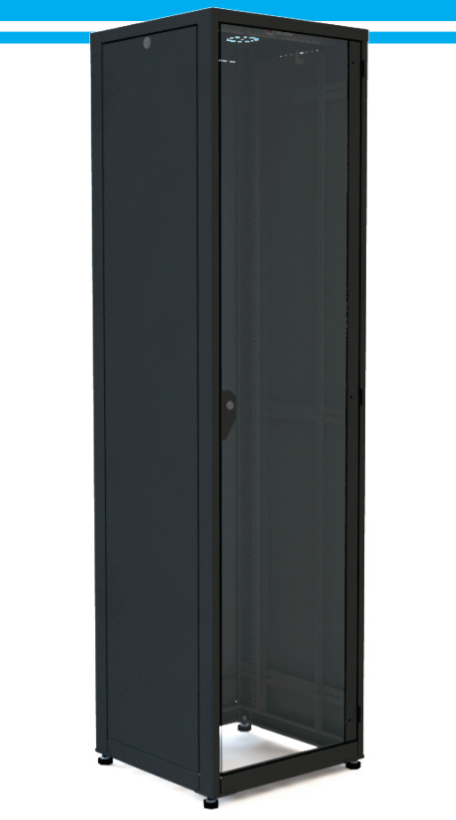
\includegraphics[height=5cm]{cont-mic.png}
            \caption{Modelo de rack utilizado de container para sistema da microrrede (disponível em: http://www.coretlc.com.br/).}
            \label{fig:cont-mod-mic}
        \end{subfigure}
        %\hspace*{\fill}
        \begin{subfigure}{0.48\linewidth}
            \centering
            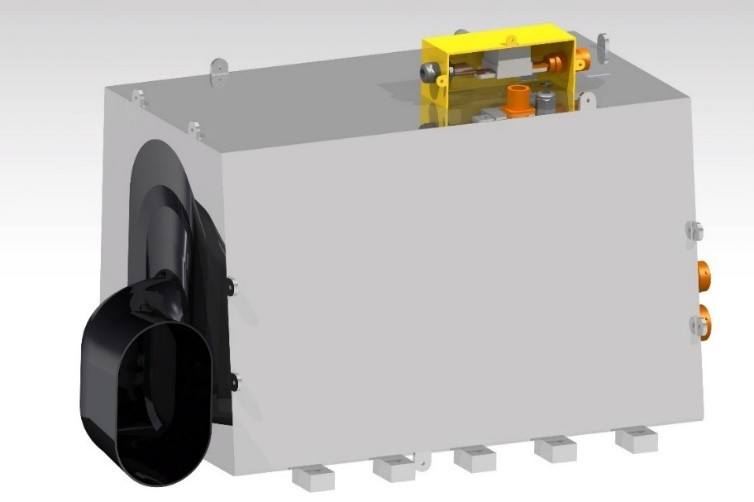
\includegraphics[height=5cm]{cont-vee.jpg}
            \caption{Rederização do container completo do veículo elétrico.}
            \label{fig:cont-mod-vee}
        \end{subfigure}
        \caption{Containeres utilizados}
        \label{fig:conts}
    \end{figure}

%=====================================================

\section{Conexões, plugs de manutenção e HVD}

    São o grupo de todas as conexões elétricas de alta tensão (\textit{High Voltage – HV}) e de baixa tensão (\textit{Low Voltage – LV}) entre dois sistemas quaisquer. Plugs de manutenção são conectores específicos para a conexão de potência entre os Segmentos, no veículo, e entre packs, na microrrede. Já o \textit{HV Disconnect (HVD)} é um sistema exclusivo do veículo elétrico, sendo o elemento fisicamente removível que permite a separação de um dos polos do sistema TS. É usado em casos de emergência para prover a separação elétrica e interromper o circuito de potência do carro. Entre os requerimentos mais importantes destes sistemas estão os cuidados que se deve ter com o isolamento elétrico e na escolha dos materiais, além de padrões de cores e a proibição do uso de estanho para conexão em sistemas de potência.

    Para a escolha dos conectores a serem utilizados foi levado em conta, além de todos os requerimentos, as necessidades e particularidades de cada conexão. Dois tipos principais de conexão são utilizados no acumulador: conexões de placa para cabo e de painel para cabo. Além disso, são usados conectores de potência para a transmissão de energia entre as células e o sistema que utilizará a energia. Dez padrões diferentes de conectores foram utilizados em mais de 50 conectores por sistema.

%=====================================================

\section{Medidor de energia}

    É também um sistema exclusivo do veículo, unicamente usado para que a entidade organizadora da competição possa medir a tensão e o consumo de energia do sistema de tração (TS). Ele é provido pelo próprio organizador da competição. Para o funcionamento do medidor de energia deve ser apenas observado o que está apontado no manual dele, fornecido pela organização da competição. Sendo que no projeto de integração do sistema isso já foi observado.

%=====================================================

\section{Fusíveis e fusível principal}

    Fusíveis é o grupo de todos os dispositivos de proteção contra sobrecorrente em ambos os sistemas HV e LV. É usado para proteger os sistemas elétricos de sobrecorrente e aquecimento dos cabos e componentes, que podem levar a queimaduras e até incêndios. Já o fusível principal está posicionado no caminho principal de corrente do acumulador e tem a função de proteger cabos, conexões, o inversor (no carro) e o conversor CC-CC (na microrrede). Entre os principais requerimentos estão aspectos do correto dimensionamento e sua montagem física. 

    Na montagem do acumulador do veículo elétrico foram ainda utilizadas conexões fusíveis para cada célula em paralelo, sendo essa um recorte na chapa de níquel que faz a conexão. Já o fusível principal foi dimensionado para corrente máxima do sistema, sendo o da microrrede de 125 A e do veículo elétrico de 225 A. Eles têm também a classificação de tensão em níveis distintos, a microrrede em 650 V e o veículo elétrico em 500 V. Ambos são fusíveis de atuação rápida próprios para a proteção de dispositivos semicondutores, como conversores e inversores.

%=====================================================

\section{Relés de isolamento do acumulador (AIRs)}

    É o dispositivo de separação de ambos os polos do Acumulador, usado para separar eletricamente todo o sistema energizado da bateria com o exterior em qualquer momento de emergência ou que não esteja sendo utilizado. Dentre os requerimentos estão aspectos do dimensionamento e a necessidade de haver um por polo do acumulador.

    No caso do veículo elétrico foi escolhido o contator com a bobina mais energeticamente eficiente do mercado. Isso com a função de reduzir o tamanho da bateria de baixa tensão do carro e por consequência diminuir o peso. Os contatores utilizados na microrrede foram os mesmos usados no ano de 2019 no carro da equipe UFPR Formula, com a principal função de reduzir os custos na implantação do sistema.

%=====================================================

\section{Circuitos de pré-carga e descarga}

    O circuito de pré-carga carrega os capacitores do inversor (no carro) e do conversor CC-CC (na microrrede) antes de fechar os relés de isolamento do acumulador (AIRs) para a conexão do acumulador com o conversor. Já o circuito de descarga descarrega esses mesmos capacitores quando os AIRs são abertos. Os requerimentos mais importantes são: é necessário carregar os capacitores ate 90\% da tensão do acumulador antes dos AIRs fecharem e é necessário que a tensão dos capacitores abaixe de 60 V DC em menos de 5 s após os AIRs abrirem

    Na microrrede ambos os circuitos já estão implementados nos circuitos do conversor CC-CC, então não há necessidade de fazer no acumulador. Já no veículo elétrico esse sistema fica dentro do container. São compostos de um relé e um resistor em cada circuito, a diferenciação é feita apenas nas conexões, no tipo do relé (normalmente aberto para o circuito de pré-carga e normalmente fechado para o circuito de descarga) e na sequência de ativação. Além disso, todos os circuitos foram projetados para funcionarem de forma segura e confiável.

%=====================================================

\section{Circuito Shutdown}

    É o circuito que carrega diretamente a corrente que realiza a ativação dos Relés de isolamento do acumulador (AIRs), passando por botões, \textit{switches}, \textit{interlocks} e \textit{latches}. É usado para abrir os relés em qualquer situação de emergência ou falha de sistemas de segurança. Dentre os requerimentos mais importantes está a lista dos itens necessários, sendo esses, dentro do container, o IMD, AMS e os respectivos \textit{interlocks} dos conectores.

%=====================================================

\section{Dispositivo de monitoramento do isolamento (IMD)}

    É um dispositivo exclusivo do carro, que mede a resistência de isolamento entre o sistema de alta tensão (\textit{High Voltage System – HVS}) e o sistema de baixa tensão aterrado (\textit{Grounded Low Voltage System – GLVS}). É usado para abrir o Circuito Shutdown em qualquer momento que houver falha de isolamento, que representaria risco para outros sistemas do carro e qualquer pessoa próxima ao expor eles à alta tensão (HV). Nos requerimentos já está definido o modelo a ser utilizado, restando o trabalho de fazer o correto dimensionamento dos seus parâmetros, que foram feitos para manter o tempo máximo para ativação abaixo do indicado nos requerimentos.

%=====================================================

\section{Sistema de gerenciamento do acumulador (AMS)}

    O sistema de gerenciamento do acumulador, conhecido por AMS ou BMS, mede e monitora todos os parâmetros das células dentro do Acumulador, mantendo-as na região de operação indicada pela fabricante e listadas nos requerimentos. É usado para medir a tensão, corrente e temperatura das células, mantendo comunicação com os usuários (inversor, conversor CC-CC, piloto ou operador do sistema) e tendo a capacidade de abrir o Circuito \textit{Shutdown} em casos de emergência. Dentre os requerimentos estão vários aspectos de projetos de PCB para alta tensão, cuidados nas conexões e a listagem dos parâmetros que devem ser verificados.

    Como apresentado na discussão sobre segurança de células de íons de lítio, o AMS é o principal sistema responsável pelo correto funcionamento do acumulador. No projeto da microrrede foi utilizado um modelo comercial, o Orion BMS 2. Este é um sistema centralizado e que conta com medições de tensão, corrente e temperatura, além de fazer a estimativa de estado de carga das células e outros parâmetros de forma muito confiável. Já no veículo elétrico, o projeto de um BMS foi feito inteiro pela equipe UFPR Formula. Este tinha por função ser mais compacto e flexível que um sistema comercial. Assim, foi possível que o projeto do BMS se integrasse no projeto dos módulos do acumulador, aumentando a confiabilidade das medições e diminuindo a quantidade de cabos. Cada placa de medição conta com a capacidade de medir a tensão e temperatura de 12 células em série, os dados são então mandados para um microcontrolador central via comunicação SPI isolada. No microcontrolador são feitas as estimativas de estado de carga e os cálculos para limitação de corrente, além da comunicação externa com sistemas de telemetria, com o inversor e com o carregador.

%=====================================================

\section{Carregador e circuito \textit{Shutdown} de carga}

    É o dispositivo usado para prover energia elétrica com a função de carregar as células do Acumulador. Pelo fato de o conversor CC-CC já realizar essa função na microrrede, este é um sistema exclusivo do carro. Já o circuito \textit{Shutdown} de carga é similar ao Circuito \textit{Shutdown}, mas é usado no momento da carga, por isso é também um sistema exclusivo do carro. Todos os requerimentos acima continuam válidos para o momento da carga, além disso, é necessário que o carregador tenha certificação de padrão reconhecido, no caso, no modelo utilizado, o CE.

    O modelo usado foi o mesmo utilizado nos últimos anos no veículo elétrico, mas dessa vez, para fazer a carga os segmentos são separados, assim, um carregador de baixa tensão (máximo 99 V do modelo utilizado) pode realizar a carga de um acumulador com tensão bem superior. Essa escolha se deve principalmente pelo fato do sistema de carga ser um componente muito caro, e como medida de redução de custos foi utilizado o mesmo que já havia sido adquirido.		% resultados
\chapter{Conclusões}
\label{cap:exemplos}

%=====================================================

O principal objetivo desse trabalho foi efetuar uma pesquisa sobre o uso de sistemas de armazenamento de energia em microrredes e veículos elétricos para o desenvolvimento de um projeto completo e seguro.

Os sistemas da microrrede e do veículo elétrico foram estudados, além disso, também os principais componentes tiveram seu funcionamento investigado. Com isso foi possível verificar requisitos dos sistemas que integrariam diretamente com as baterias. Várias tecnologias de sistemas de armazenamento de energia foram estudadas, com isso foi possível ter um panorama geral do mercado e dos usos atuais e futuros.

Verificou-se que a tecnologia de baterias de íons de lítio é atualmente a que apresenta as maiores densidades de energia e potência, sendo por isso escolhida para o uso nesse projeto. Seu funcionamento foi estudado, assim como todos os aspectos de segurança, para definir então a melhor forma de operação e requisitos de projeto.

Foi definida uma metodologia de projetos, que a partir daí foi desenvolvido. O sistema de armazenamento foi separado em vários subsistemas e requerimentos individuais foram definidos. Foi desenvolvido o projeto de arquitetura e integração dos sistemas, para mostrar como cada parte seria integrada no projeto, assim como prover documentação para integração externa. Na fase de especificação dos componentes, estes foram definidos de forma a proporcionar uma descrição completa para as compras e manufatura dos sistemas.

O presente trabalho é uma referência para futuros trabalhos dentro da Universidade Federal do Paraná e da equipe UFPR Formula, para que seja feita uma correta operação e manutenção dos sistemas. Para a finalização, ainda é necessário que a fase de manufatura seja realizada, que foi atrasada pela pandemia de COVID-19, além de todos os testes de componente, integração e sistema, tanto do armazenamento para a microrrede quanto do veículo elétrico.
		% conclusão

%=====================================================

% Estilos de bibliografia recomendados (só descomentar um estilo!)
% Mais infos: https://pt.sharelatex.com/learn/Bibtex_bibliography_styles
%
% ATENÇÃO: evite usar \cite{}; prefira \citep{} e \citet{}
%
\bibliographystyle{apalike-ptbr}	% [Maziero et al., 2006]
%\bibliographystyle{alpha}		% [Maz06]
%\bibliographystyle{plainnat}		% vide Google "LaTeX Natbib"
%\bibliographystyle{plain}		% [1] ordem alfabética
%\bibliographystyle{unsrt}		% [1] ordem de uso no texto

% no estilo "unsrt", evita que citações nos índices sejam consideradas
%\usepackage{notoccite}

% base de bibliografia (BibTeX)
\bibliography{referencias}
%\bibliography{file1,file2,file3} % se tiver mais de um arquivo BibTeX

%=====================================================

% inclusão de apêndices
%\appendix

% inclusão de apêndice
%\chapter{Exemplo de anexo}

%=====================================================

Os apêndices são uma extensão do texto, destacados deste para evitar descontinuidade na sequência lógica ou alongamento excessivo de determinado assunto ou tópico secundário dentro dos capítulos da dissertação ou da tese. São contribuições que servem para esclarecer, complementar, provar ou confirmar as ideias apresentadas no texto dos capítulos e que são importantes para a compreensão dos mesmos.

Todos os apêndices devem vir após as referências bibliográficas e devem ser enumerados por letras maiúsculas (A, B, C, ...).

%=====================================================

\section{Uma Seção}

\lipsum[20-23]

%=====================================================

\subsection{Uma sub-Seção}

\lipsum[30-33]

%=====================================================

\subsection{Outra sub-Seção}

Exemplo de lista simples com dois níveis: Exemplo de lista simples com dois níveis: Exemplo de lista simples com dois níveis: Exemplo de lista simples com dois níveis: Exemplo de lista simples com dois níveis: Exemplo de lista simples com dois níveis: Exemplo de lista simples com dois níveis: Exemplo de lista simples com dois níveis: Exemplo de lista simples com dois níveis.

\begin{itemize}

\item Banana, Banana, Banana, Banana, Banana, Banana, Banana, Banana, Banana, Banana, Banana, Banana, Banana, Banana, Banana, Banana, Banana, Banana, Banana, Banana, Banana, Banana, Banana, Banana.

\begin{itemize}

\item Caturra, Caturra, Caturra, Caturra, Caturra, Caturra, Caturra, Caturra, Caturra, Caturra, Caturra, Caturra, Caturra, Caturra, Caturra, Caturra, Caturra, Caturra, Caturra.

\item da Terra, da Terra, da Terra, da Terra, da Terra, da Terra, da Terra, da Terra, da Terra, da Terra, da Terra, da Terra, da Terra, da Terra, da Terra, da Terra, da Terra, da Terra.

\end{itemize}

\item Laranja, Laranja, Laranja, Laranja, Laranja, Laranja, Laranja, Laranja, Laranja, Laranja, Laranja, Laranja, Laranja, Laranja, Laranja, Laranja.

\begin{itemize}

\item Bahia, Bahia, Bahia, Bahia, Bahia, Bahia, Bahia, Bahia, Bahia, Bahia, Bahia, Bahia, Bahia, Bahia, Bahia, Bahia, Bahia, Bahia.

\item Lima, Lima, Lima, Lima, Lima, Lima, Lima, Lima, Lima, Lima, Lima, Lima, Lima, Lima, Lima, Lima, Lima, Lima, Lima, Lima, Lima, Lima, Lima, Lima, Lima, Lima, Lima, Lima, Lima.

\end{itemize}

\end{itemize}

Exemplo de lista numerada com dois níveis: Exemplo de lista numerada com dois níveis: Exemplo de lista numerada com dois níveis: Exemplo de lista numerada com dois níveis: Exemplo de lista numerada com dois níveis: Exemplo de lista numerada com dois níveis: Exemplo de lista numerada com dois níveis: Exemplo de lista numerada com dois níveis.

\begin{enumerate}

\item Banana, Banana, Banana, Banana, Banana, Banana, Banana, Banana, Banana, Banana, Banana, Banana, Banana, Banana, Banana, Banana, Banana, Banana, Banana, Banana, Banana, Banana, Banana, Banana.

\begin{enumerate}

\item Caturra, Caturra, Caturra, Caturra, Caturra, Caturra, Caturra, Caturra, Caturra, Caturra, Caturra, Caturra, Caturra, Caturra, Caturra, Caturra, Caturra, Caturra, Caturra.

\item da Terra, da Terra, da Terra, da Terra, da Terra, da Terra, da Terra, da Terra, da Terra, da Terra, da Terra, da Terra, da Terra, da Terra, da Terra, da Terra, da Terra, da Terra.

\end{enumerate}

\item Laranja, Laranja, Laranja, Laranja, Laranja, Laranja, Laranja, Laranja, Laranja, Laranja, Laranja, Laranja, Laranja, Laranja, Laranja, Laranja.

\begin{enumerate}

\item Bahia, Bahia, Bahia, Bahia, Bahia, Bahia, Bahia, Bahia, Bahia, Bahia, Bahia, Bahia, Bahia, Bahia, Bahia, Bahia, Bahia, Bahia.

\item Lima, Lima, Lima, Lima, Lima, Lima, Lima, Lima, Lima, Lima, Lima, Lima, Lima, Lima, Lima, Lima, Lima, Lima, Lima, Lima, Lima, Lima, Lima, Lima, Lima, Lima, Lima, Lima, Lima.

\end{enumerate}

\end{enumerate}

Exemplo de lista descritiva com dois níveis: Exemplo de lista descritiva com dois níveis: Exemplo de lista descritiva com dois níveis: Exemplo de lista descritiva com dois níveis: Exemplo de lista descritiva com dois níveis: Exemplo de lista descritiva com dois níveis: Exemplo de lista descritiva com dois níveis: Exemplo de lista descritiva com dois níveis: Exemplo de lista descritiva com dois níveis.

\begin{description}

\item [Banana]: Banana, Banana, Banana, Banana, Banana, Banana, Banana, Banana, Banana, Banana, Banana, Banana, Banana, Banana, Banana, Banana, Banana, Banana, Banana, Banana, Banana, Banana, Banana.

\begin{description}

\item [Caturra]: Caturra, Caturra, Caturra, Caturra, Caturra, Caturra, Caturra, Caturra, Caturra, Caturra, Caturra, Caturra, Caturra, Caturra, Caturra, Caturra, Caturra, Caturra.

\item [da Terra]: da Terra, da Terra, da Terra, da Terra, da Terra, da Terra, da Terra, da Terra, da Terra, da Terra, da Terra, da Terra, da Terra, da Terra, da Terra, da Terra, da Terra.

\end{description}

\item [Laranja]: Laranja, Laranja, Laranja, Laranja, Laranja, Laranja, Laranja, Laranja, Laranja, Laranja, Laranja, Laranja, Laranja, Laranja, Laranja.

\begin{description}

\item [Bahia]: Bahia, Bahia, Bahia, Bahia, Bahia, Bahia, Bahia, Bahia, Bahia, Bahia, Bahia, Bahia, Bahia, Bahia, Bahia, Bahia, Bahia.

\item [Lima]: Lima, Lima, Lima, Lima, Lima, Lima, Lima, Lima, Lima, Lima, Lima, Lima, Lima, Lima, Lima, Lima, Lima, Lima, Lima, Lima, Lima, Lima, Lima, Lima, Lima, Lima, Lima, Lima.

\end{description}

\end{description}

%=====================================================


% inclusão de apêndice
%\chapter{Testes de alinhamento de listas}

%=====================================================

\section{Outra seção}

Exemplo de lista simples com dois níveis: Exemplo de lista simples com dois níveis: Exemplo de lista simples com dois níveis: Exemplo de lista simples com dois níveis: Exemplo de lista simples com dois níveis: Exemplo de lista simples com dois níveis: Exemplo de lista simples com dois níveis: Exemplo de lista simples com dois níveis: Exemplo de lista simples com dois níveis.

\begin{itemize}

\item Banana, Banana, Banana, Banana, Banana, Banana, Banana, Banana, Banana, Banana, Banana, Banana, Banana, Banana, Banana, Banana, Banana, Banana, Banana, Banana, Banana, Banana, Banana, Banana.

\begin{itemize}

\item Caturra, Caturra, Caturra, Caturra, Caturra, Caturra, Caturra, Caturra, Caturra, Caturra, Caturra, Caturra, Caturra, Caturra, Caturra, Caturra, Caturra, Caturra, Caturra.

\item da Terra, da Terra, da Terra, da Terra, da Terra, da Terra, da Terra, da Terra, da Terra, da Terra, da Terra, da Terra, da Terra, da Terra, da Terra, da Terra, da Terra, da Terra.

\end{itemize}

\item Laranja, Laranja, Laranja, Laranja, Laranja, Laranja, Laranja, Laranja, Laranja, Laranja, Laranja, Laranja, Laranja, Laranja, Laranja, Laranja.

\begin{itemize}

\item Bahia, Bahia, Bahia, Bahia, Bahia, Bahia, Bahia, Bahia, Bahia, Bahia, Bahia, Bahia, Bahia, Bahia, Bahia, Bahia, Bahia, Bahia.

\item Lima, Lima, Lima, Lima, Lima, Lima, Lima, Lima, Lima, Lima, Lima, Lima, Lima, Lima, Lima, Lima, Lima, Lima, Lima, Lima, Lima, Lima, Lima, Lima, Lima, Lima, Lima, Lima, Lima.

\end{itemize}

\end{itemize}

Exemplo de lista numerada com dois níveis: Exemplo de lista numerada com dois níveis: Exemplo de lista numerada com dois níveis: Exemplo de lista numerada com dois níveis: Exemplo de lista numerada com dois níveis: Exemplo de lista numerada com dois níveis: Exemplo de lista numerada com dois níveis: Exemplo de lista numerada com dois níveis.

\begin{enumerate}

\item Banana, Banana, Banana, Banana, Banana, Banana, Banana, Banana, Banana, Banana, Banana, Banana, Banana, Banana, Banana, Banana, Banana, Banana, Banana, Banana, Banana, Banana, Banana, Banana.

\begin{enumerate}

\item Caturra, Caturra, Caturra, Caturra, Caturra, Caturra, Caturra, Caturra, Caturra, Caturra, Caturra, Caturra, Caturra, Caturra, Caturra, Caturra, Caturra, Caturra, Caturra.

\item da Terra, da Terra, da Terra, da Terra, da Terra, da Terra, da Terra, da Terra, da Terra, da Terra, da Terra, da Terra, da Terra, da Terra, da Terra, da Terra, da Terra, da Terra.

\end{enumerate}

\item Laranja, Laranja, Laranja, Laranja, Laranja, Laranja, Laranja, Laranja, Laranja, Laranja, Laranja, Laranja, Laranja, Laranja, Laranja, Laranja.

\begin{enumerate}

\item Bahia, Bahia, Bahia, Bahia, Bahia, Bahia, Bahia, Bahia, Bahia, Bahia, Bahia, Bahia, Bahia, Bahia, Bahia, Bahia, Bahia, Bahia.

\item Lima, Lima, Lima, Lima, Lima, Lima, Lima, Lima, Lima, Lima, Lima, Lima, Lima, Lima, Lima, Lima, Lima, Lima, Lima, Lima, Lima, Lima, Lima, Lima, Lima, Lima, Lima, Lima, Lima.

\end{enumerate}

\end{enumerate}

Exemplo de lista descritiva com dois níveis: Exemplo de lista descritiva com dois níveis: Exemplo de lista descritiva com dois níveis: Exemplo de lista descritiva com dois níveis: Exemplo de lista descritiva com dois níveis: Exemplo de lista descritiva com dois níveis: Exemplo de lista descritiva com dois níveis: Exemplo de lista descritiva com dois níveis: Exemplo de lista descritiva com dois níveis.

\begin{description}

\item [Banana]: Banana, Banana, Banana, Banana, Banana, Banana, Banana, Banana, Banana, Banana, Banana, Banana, Banana, Banana, Banana, Banana, Banana, Banana, Banana, Banana, Banana, Banana, Banana.

\begin{description}

\item [Caturra]: Caturra, Caturra, Caturra, Caturra, Caturra, Caturra, Caturra, Caturra, Caturra, Caturra, Caturra, Caturra, Caturra, Caturra, Caturra, Caturra, Caturra, Caturra.

\item [da Terra]: da Terra, da Terra, da Terra, da Terra, da Terra, da Terra, da Terra, da Terra, da Terra, da Terra, da Terra, da Terra, da Terra, da Terra, da Terra, da Terra, da Terra.

\end{description}

\item [Laranja]: Laranja, Laranja, Laranja, Laranja, Laranja, Laranja, Laranja, Laranja, Laranja, Laranja, Laranja, Laranja, Laranja, Laranja, Laranja.

\begin{description}

\item [Bahia]: Bahia, Bahia, Bahia, Bahia, Bahia, Bahia, Bahia, Bahia, Bahia, Bahia, Bahia, Bahia, Bahia, Bahia, Bahia, Bahia, Bahia.

\item [Lima]: Lima, Lima, Lima, Lima, Lima, Lima, Lima, Lima, Lima, Lima, Lima, Lima, Lima, Lima, Lima, Lima, Lima, Lima, Lima, Lima, Lima, Lima, Lima, Lima, Lima, Lima, Lima, Lima.

\end{description}

\end{description}

%=====================================================


%=====================================================

\end{document}

%=====================================================
